%!TEX root = ../thesis.tex
% ******************************* Thesis Appendix C ********************************

\chapter{Reinterpretation in the pMSSM}

\graphicspath{{chapter-pmssm/Figs/Vector/}{chapter-pmssm/Figs/}}

The following sections show supporting material for the reinterpretation of the \onelepton search in the \gls{pmssm}, discussed in \cref{ch:pmssm}.


\section{Further validation of the simplified likelihood}

\Cref{fig:validation_simplified_full_likelihood} compares the observed CL$_s$ values obtained for the \gls{pmssm} models sampled using the various likelihoods of the \onelepton search  discussed throughout \cref{part:reinterpretation} of this thesis. In general, the observed CL$_s$ values from the simplified likelihood are closer to those obtained using the full likelihood, than the ones obtained using the single-bin likelihood (built using the discovery signal regions).

Although showing a good agreement, the CL$_s$ naturally do not match perfectly. For this reason, the simplified likelihood can only be used for models giving observed CL$_s$ moderately far away from the exclusion boundary at 0.05. Models with a CL$_s$ value too close to 0.05 need to be evaluated using the full likelihood and \textsc{Recast} for full statistical precision. The benefit of the simplified likelihood, compared to the single-bin approach using the discovery signal regions, is that, due to the improved agreement in observed CL$_s$, the range in observed CL$_s$ around 0.05 to be evaluated using the full likelihood can be chosen to be significantly narrower.
\begin{figure}[H]
\floatbox[{\capbeside\thisfloatsetup{capbesideposition={right,center},capbesidewidth=0.45\textwidth}}]{figure}[\FBwidth]
{\caption{Observed CL$_s$ values obtained for all \gls{pmssm} models sampled for different likelihood configurations of the \onelepton search. In green, the simplified likelihood discussed in \cref{ch:simplify} is compared with the full analysis likelihood. In purple, the single-bin likelihood configuration using the discovery signal regions is used.}\label{fig:validation_simplified_full_likelihood}}
{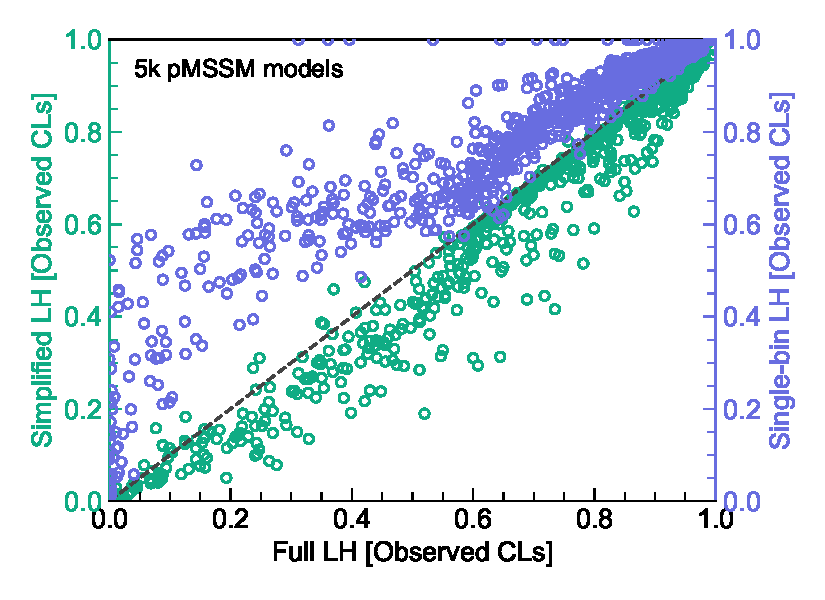
\includegraphics[width=0.5\textwidth]{fig_scatter_likelihoods}}
\end{figure}

\FloatBarrier

\section{Phenomenology of the LSP}

\Cref{fig:lsp_phenomenology_parameters} shows the \gls{lsp} type as a function of the \gls{pmssm} parameters $M_1$, $M_2$, $\mu$ and $\tan\beta$. Models with $\vert M_1\vert < \vert M_2\vert$ and $\vert M_1\vert \ll \vert\mu\vert$ tend to have an \gls{lsp} with dominant bino component, while models with $\vert M_2 \vert < \vert M_1 \vert$ and $ \vert M_2 \vert  \ll \vert\mu\vert$, have an \gls{lsp} that is mostly wino-like.
Models with $\vert\mu\vert\ll \vert M_1 \vert$ and $\vert\mu\vert\ll \vert M_2 \vert$ have mostly higgsino-like \glspl{lsp}.
%In models with mass parameters in between those edge cases, the \gls{lsp} becomes a mixed state.
The parameter $\tan\beta$ does not have a large impact on the \gls{lsp} type within the ranges sampled.

\Cref{fig:impact_electroweakinos_2D_bino_lsp} shows the fraction of models excluded by the \onelepton search in different two-dimensional projections on the electroweakino masses.
%Only models with a bino-like (left) or wino-like (right) \gls{lsp} are shown in order to highlight the different spectra. No models with a higgsino-like \gls{lsp} are shown since the \onelepton search is not sensitive to such scenarios.
Models with a bino-like \gls{lsp} tend to have nearly mass-degenerate $\charg$ and $\neutr$ and are thus close to the canonical simplified model considered in the search. Models with a wino-like \gls{lsp} have nearly mass-degenerate $\charg$ and $\lsp$. In such models, the \onelepton search can be sensitive to $\tilde{\chi}_2^\pm\neutr$ production.

 \begin{figure}[H]
	\centering
	\begin{subfigure}[b]{0.47\linewidth}
		\centering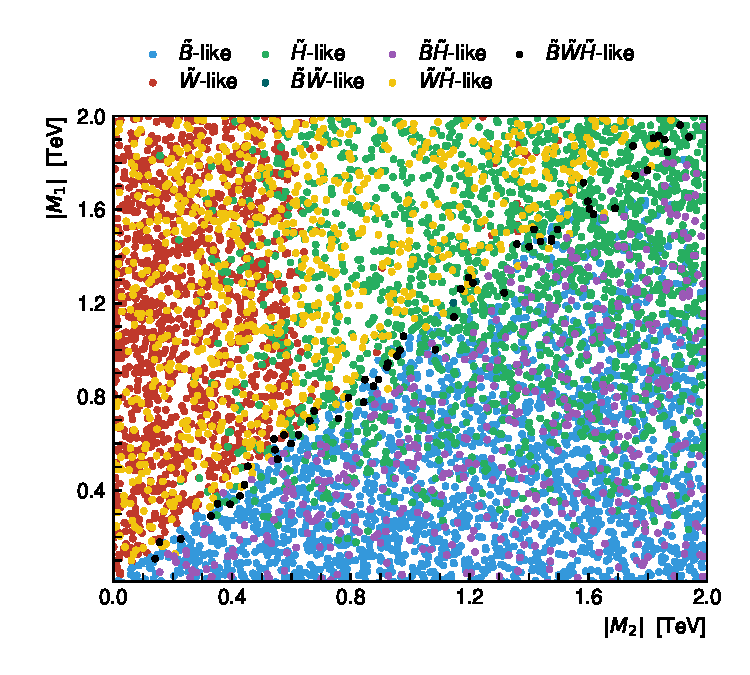
\includegraphics[width=\textwidth]{scatter/lsp_types_M1_M2}
	\end{subfigure}\hfill
	\begin{subfigure}[b]{0.47\linewidth}
		\centering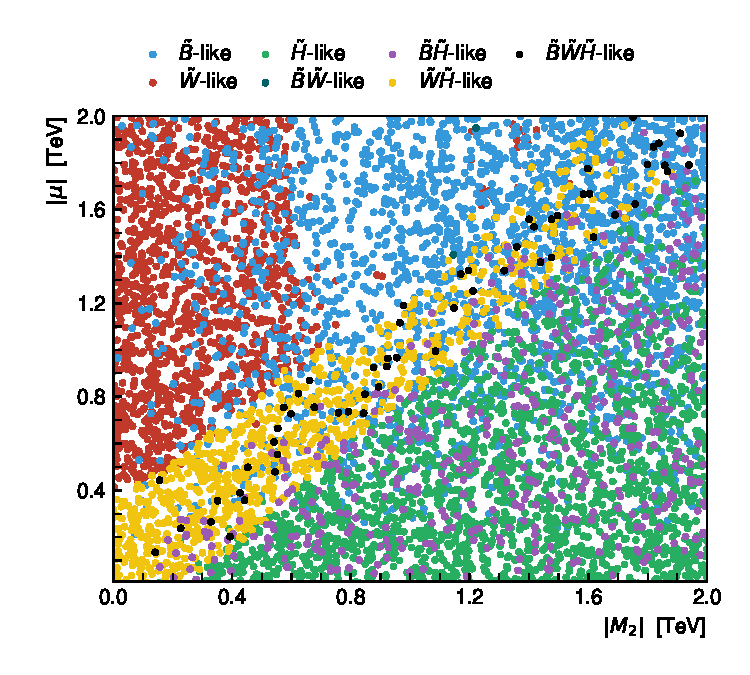
\includegraphics[width=\textwidth]{scatter/lsp_types_mu_M2}
	\end{subfigure}\hfill
	
	\vspace{-1.0em}
	\begin{subfigure}[b]{0.47\linewidth}
		\centering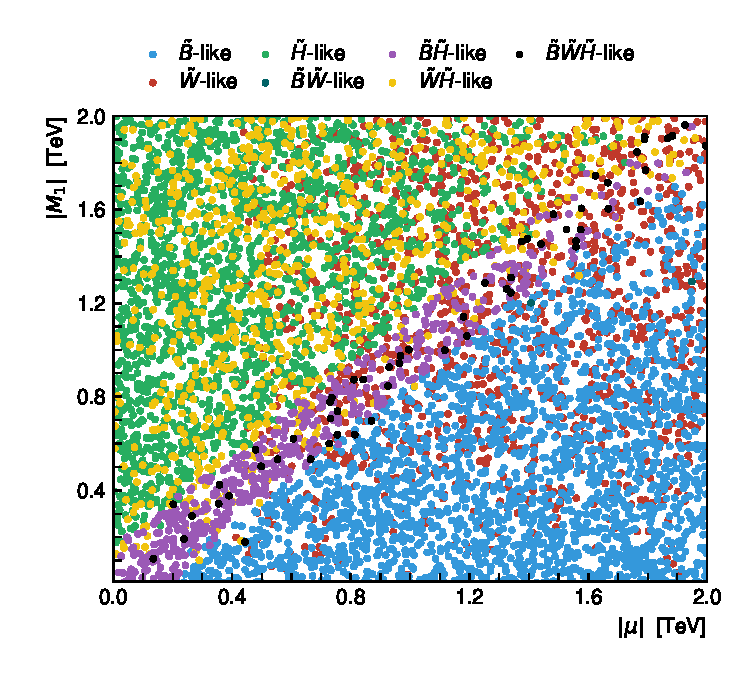
\includegraphics[width=\textwidth]{scatter/lsp_types_mu_M1}
	\end{subfigure}\hfill
	\begin{subfigure}[b]{0.47\linewidth}
		\centering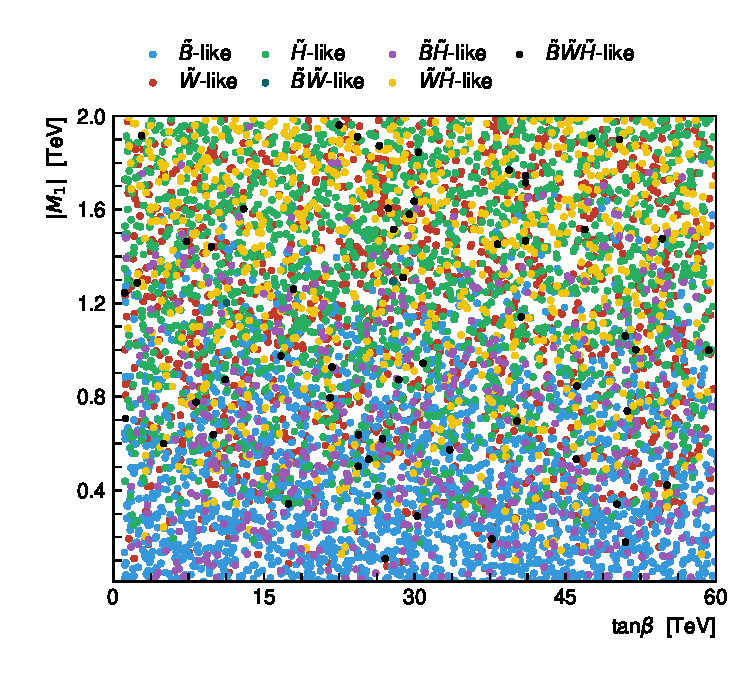
\includegraphics[width=\textwidth]{scatter/lsp_types_tanb_M1}
	\end{subfigure}\hfill
	\caption{Phenomenology of the \gls{lsp} as a function of two-dimensional projections of the \gls{pmssm} parameter space. The parameters $M_1$, $M_2$, $\mu$ and $\tan\beta$ in various projections. Each point in the plots corresponds to a unique \gls{pmssm} model sampled. The colour codes the nature of the \gls{lsp} using the definitions introduced in \cref{sec:lsp_pheno}.}
	\label{fig:lsp_phenomenology_parameters}
\end{figure}


\begin{figure}
	\centering
	\begin{subfigure}[b]{0.5\linewidth}
		\centering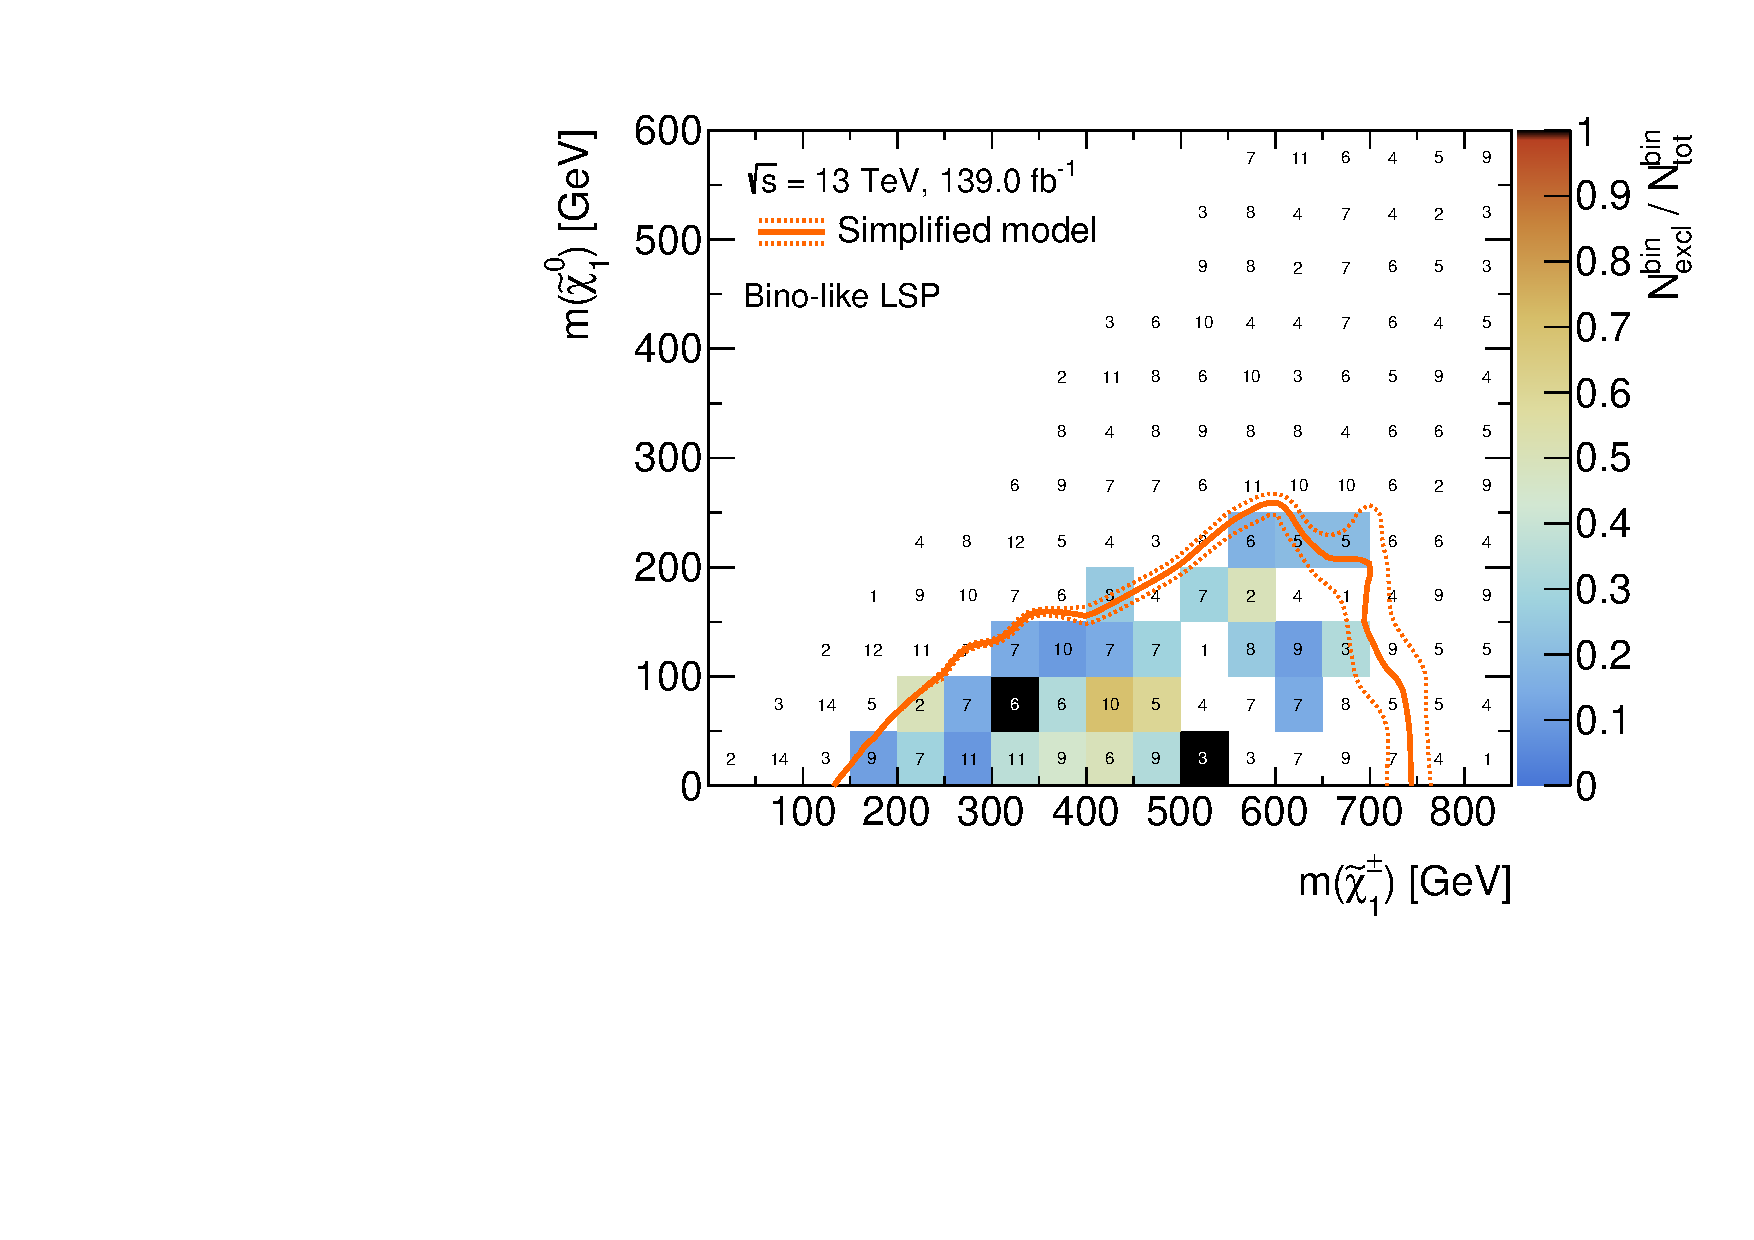
\includegraphics[width=\textwidth]{cut_bino_LSP/mchi1p_mlsp_contour}
	\end{subfigure}\hfill
	\begin{subfigure}[b]{0.5\linewidth}
		\centering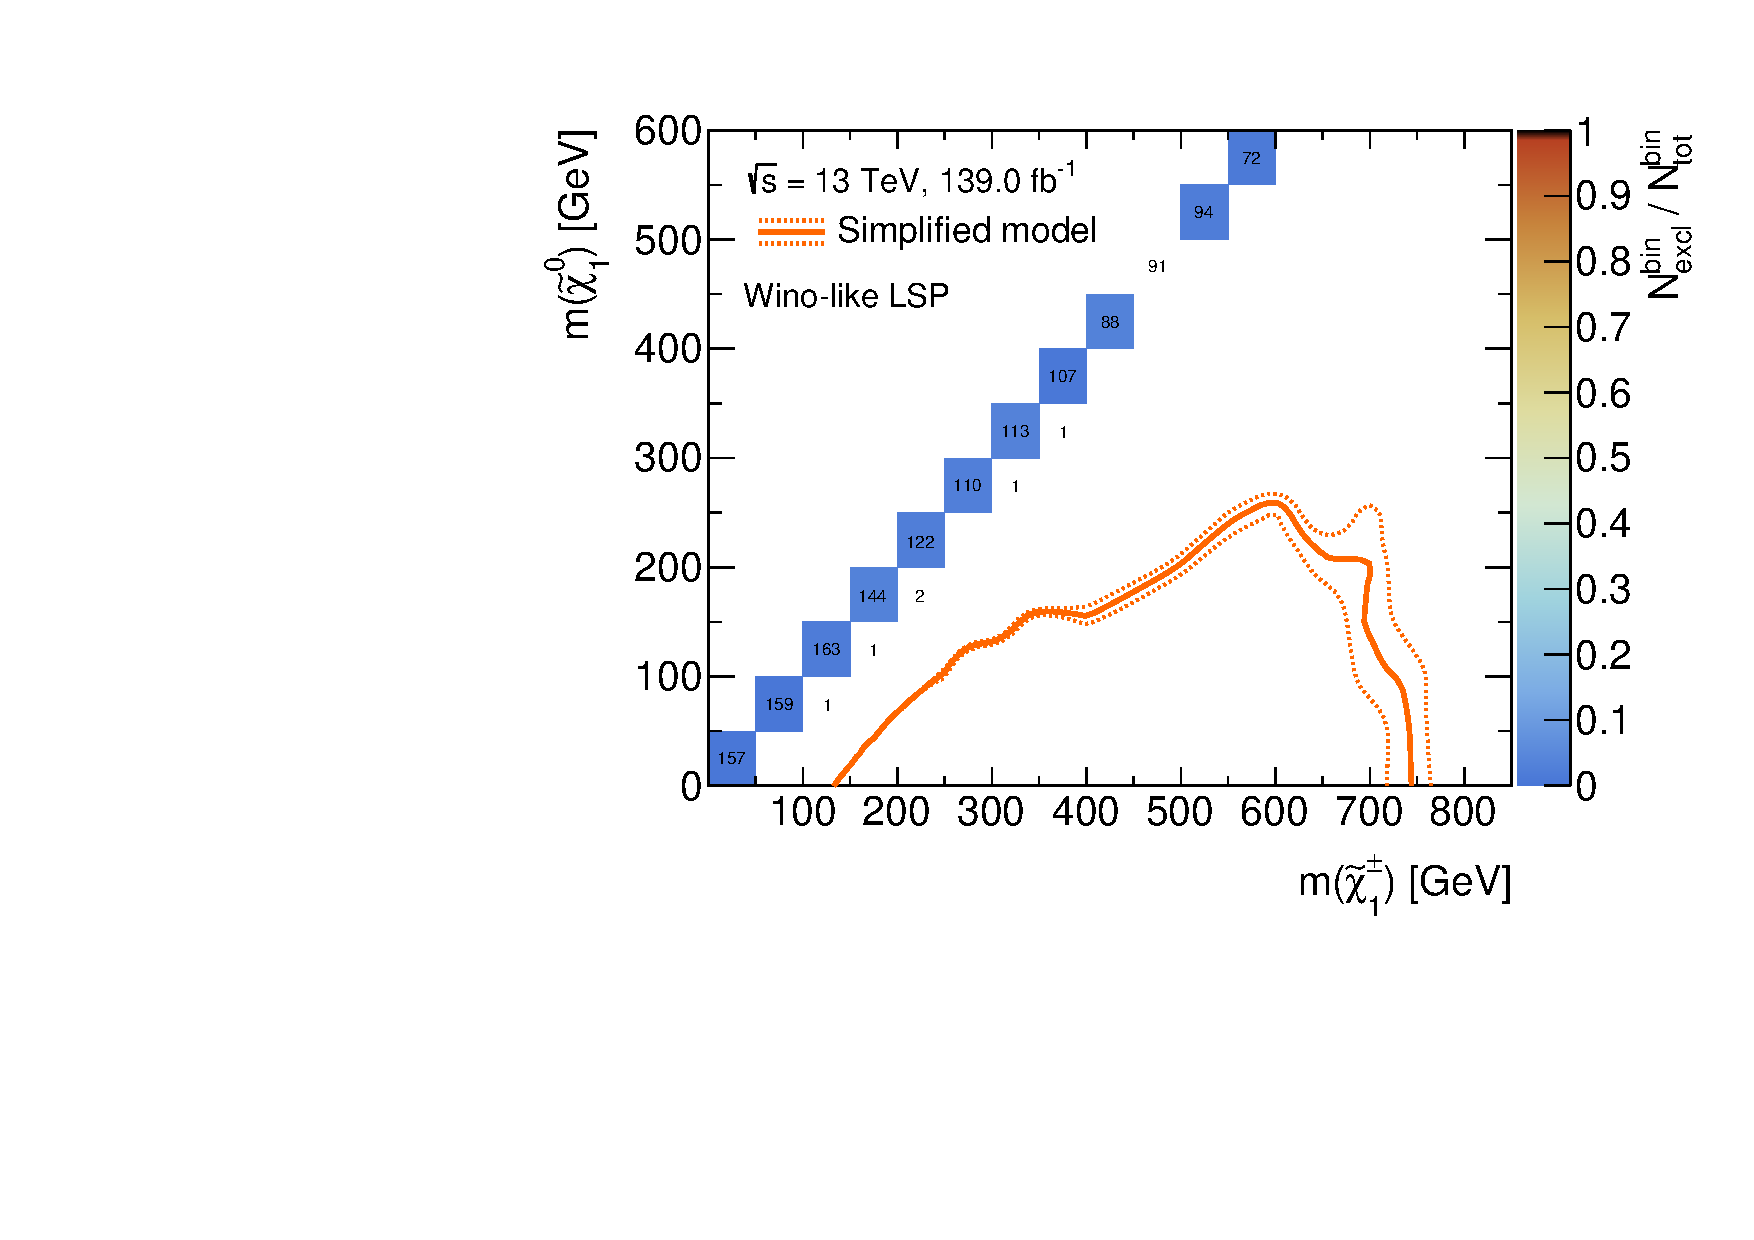
\includegraphics[width=\textwidth]{cut_wino_LSP/mchi1p_mlsp_contour}
	\end{subfigure}\hfill
	
	\begin{subfigure}[b]{0.5\linewidth}
		\centering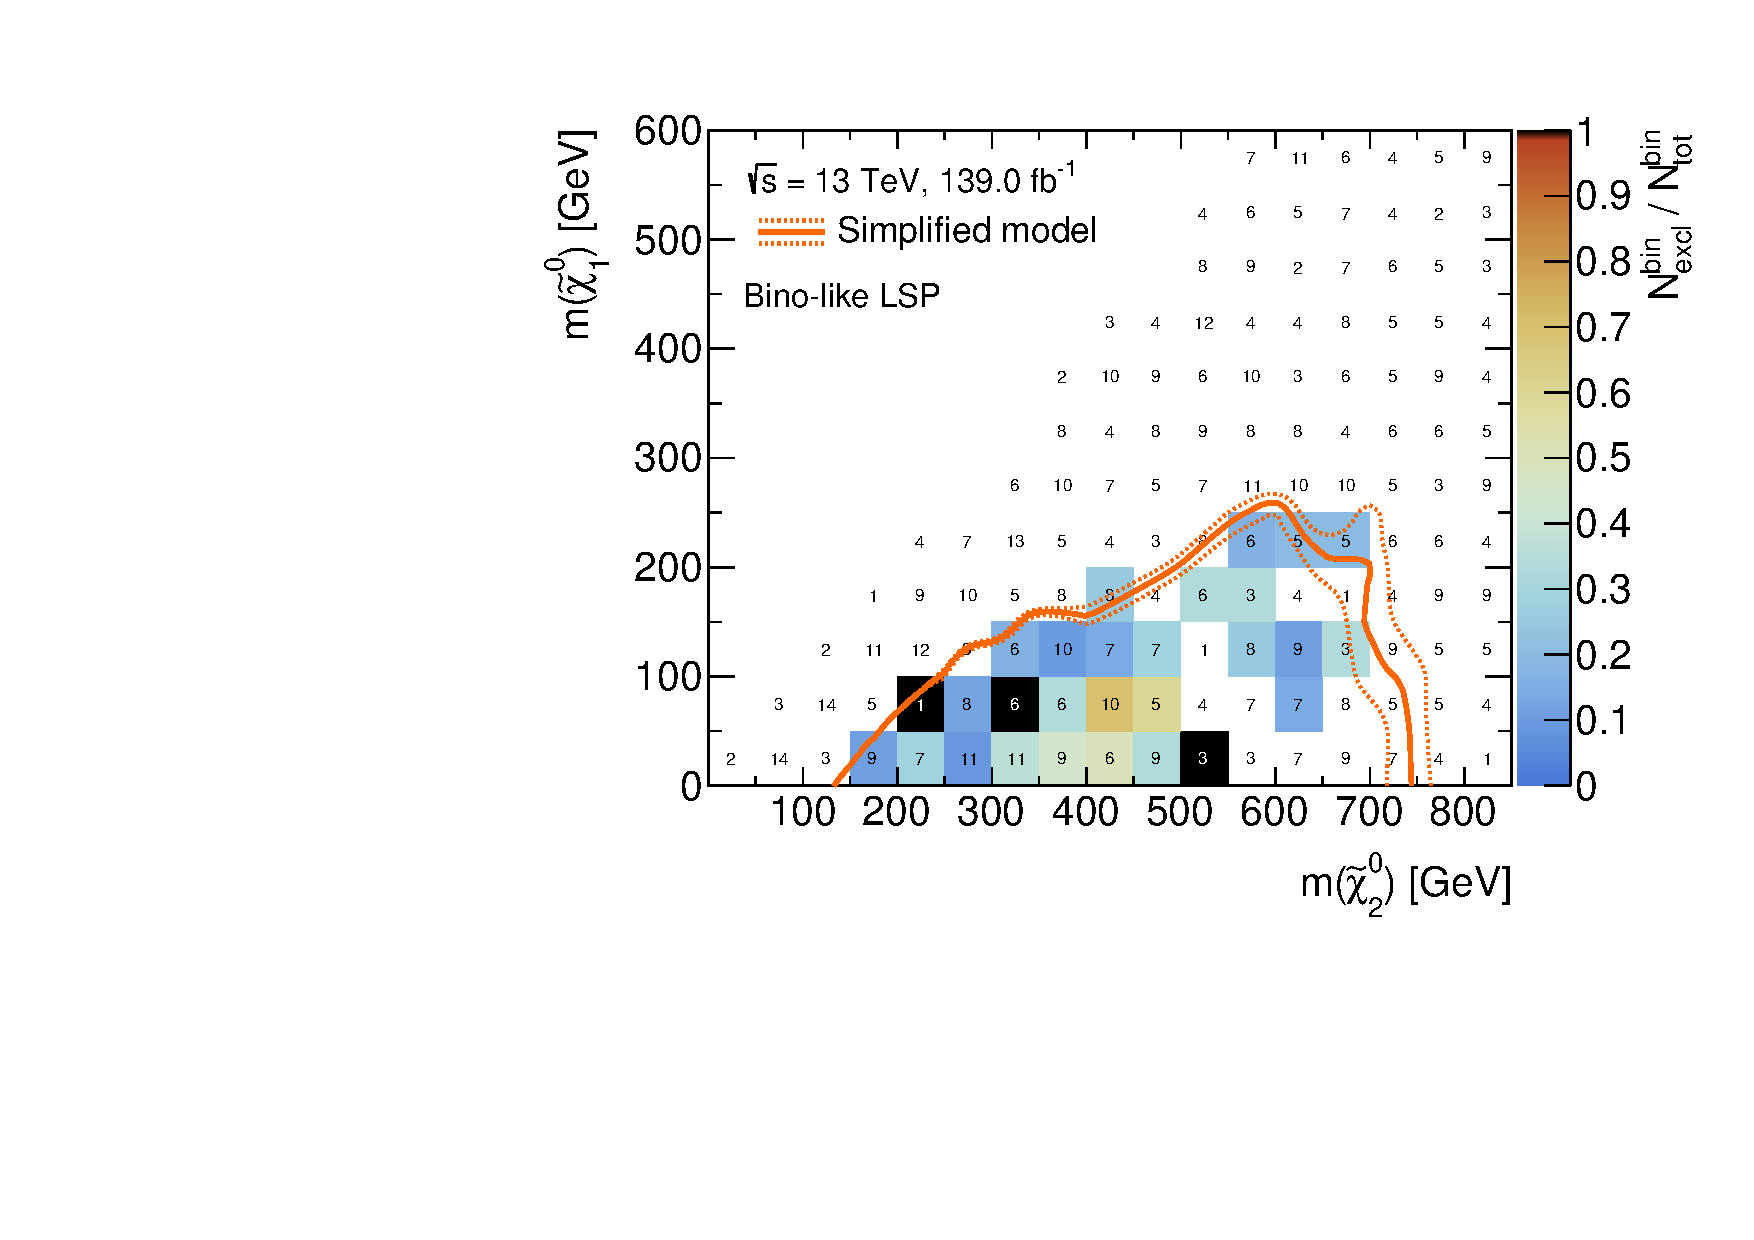
\includegraphics[width=\textwidth]{cut_bino_LSP/mchi20_mlsp_contour}
	\end{subfigure}\hfill
	\begin{subfigure}[b]{0.5\linewidth}
		\centering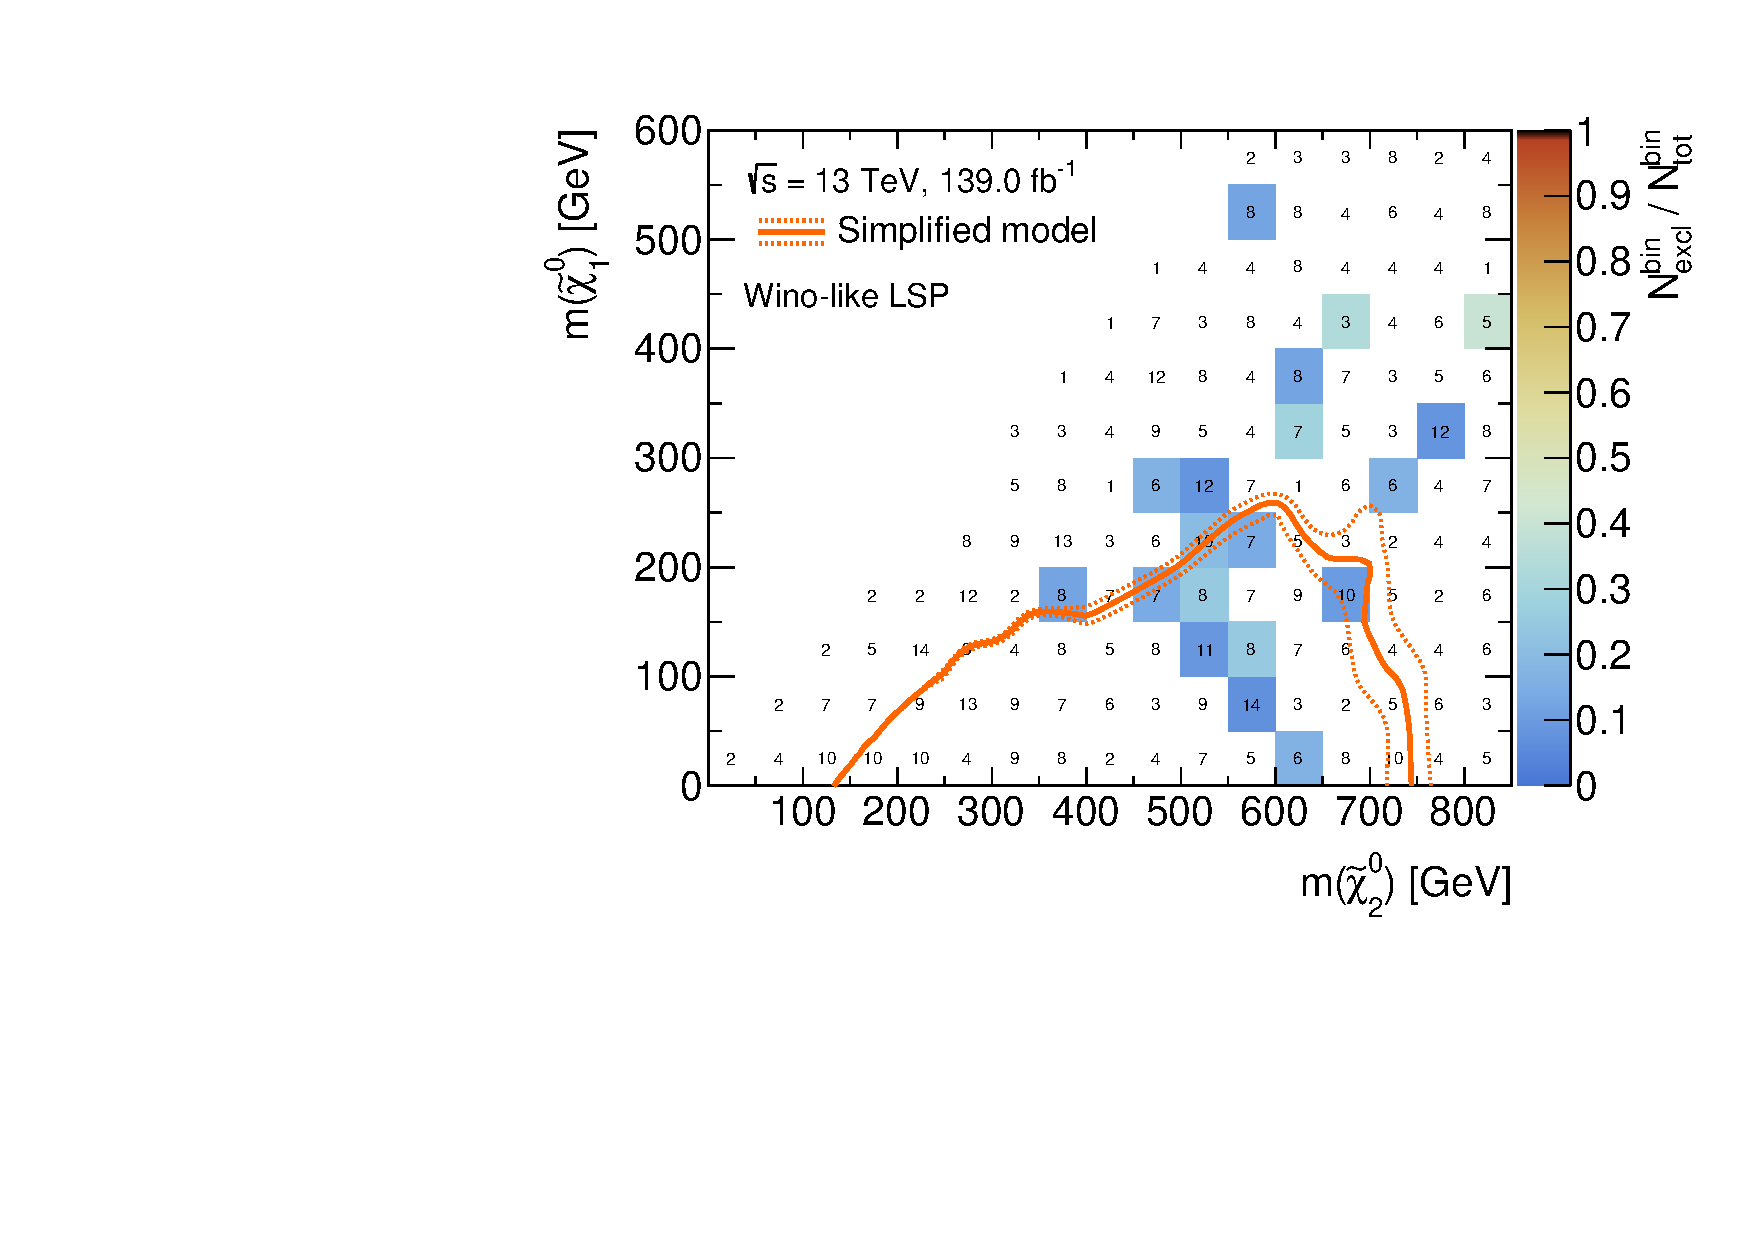
\includegraphics[width=\textwidth]{cut_wino_LSP/mchi20_mlsp_contour}
	\end{subfigure}\hfill
	
	\begin{subfigure}[b]{0.5\linewidth}
		\centering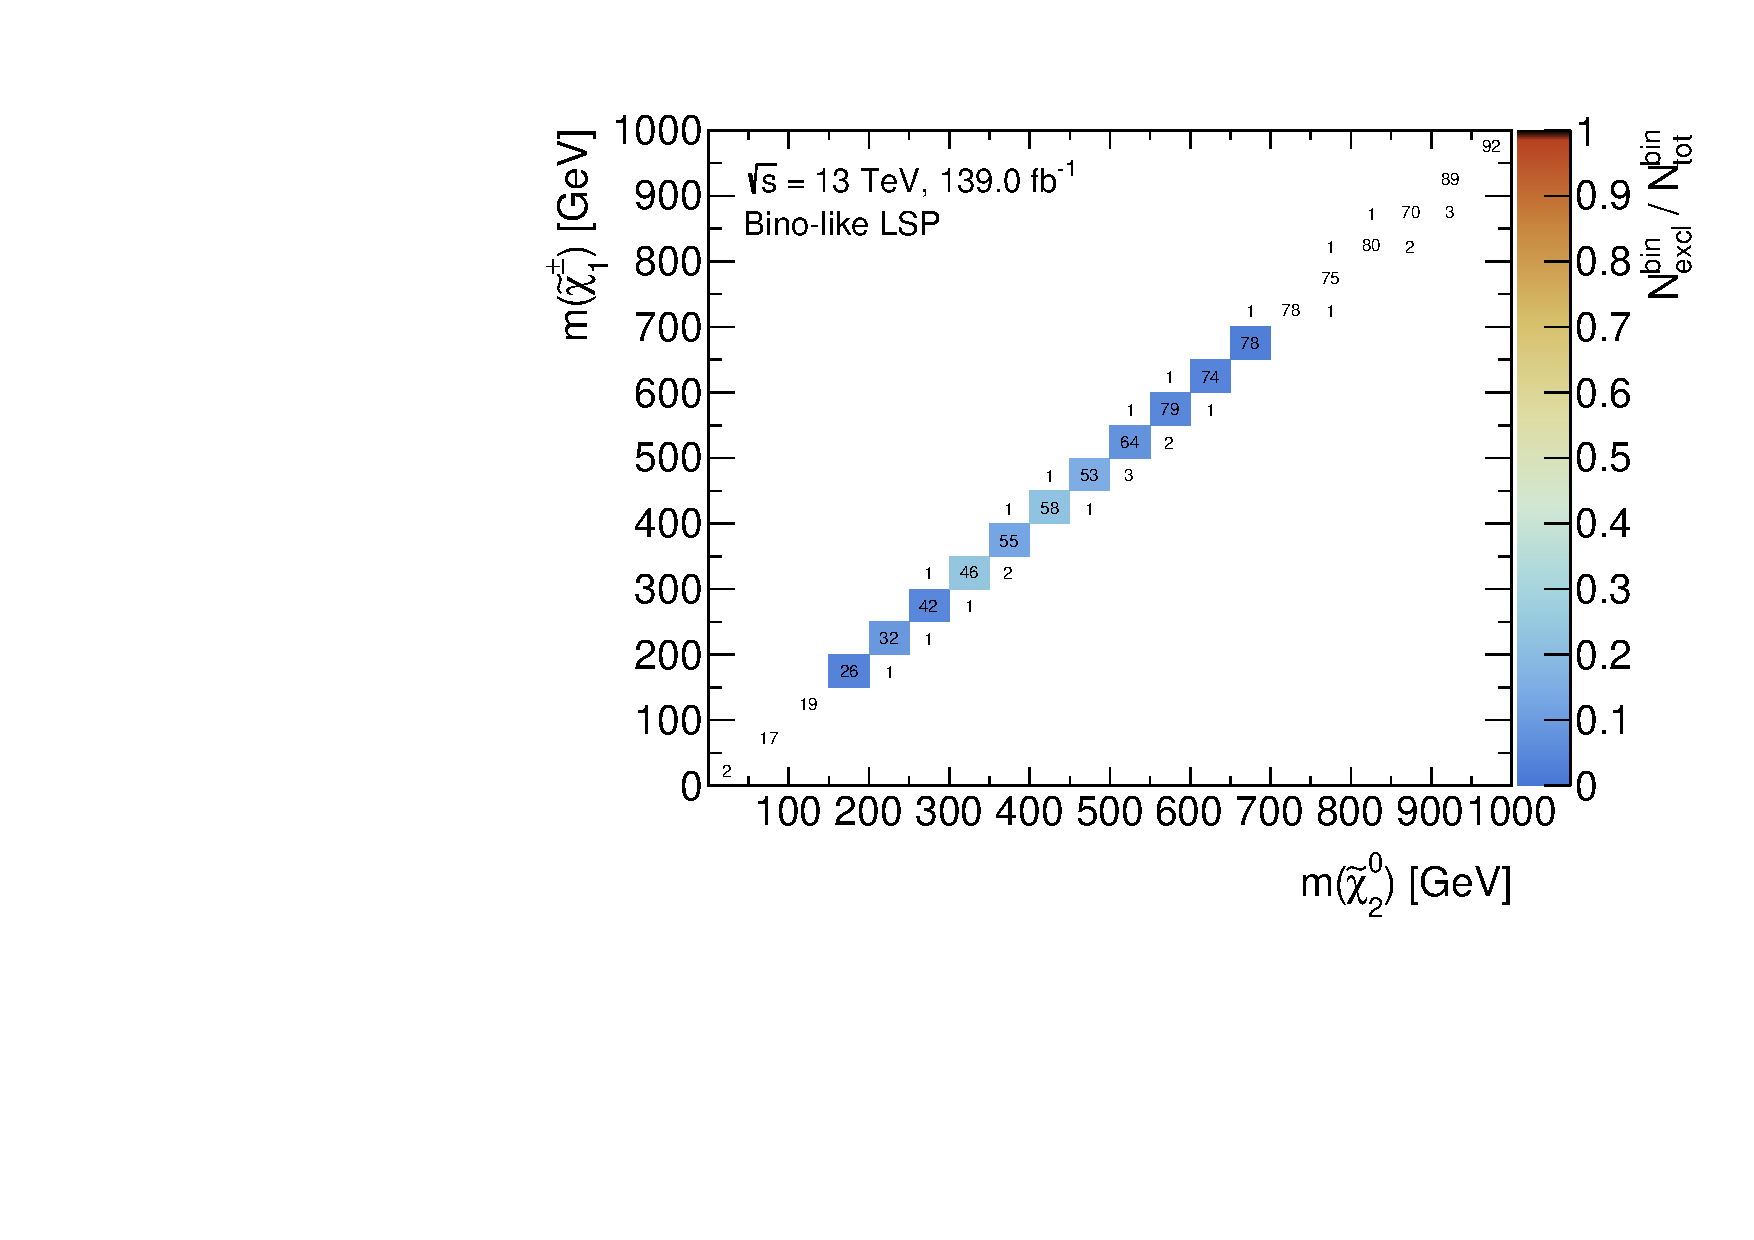
\includegraphics[width=\textwidth]{cut_bino_LSP/mchi1p_mchi20_contour}
	\end{subfigure}\hfill
	\begin{subfigure}[b]{0.5\linewidth}
		\centering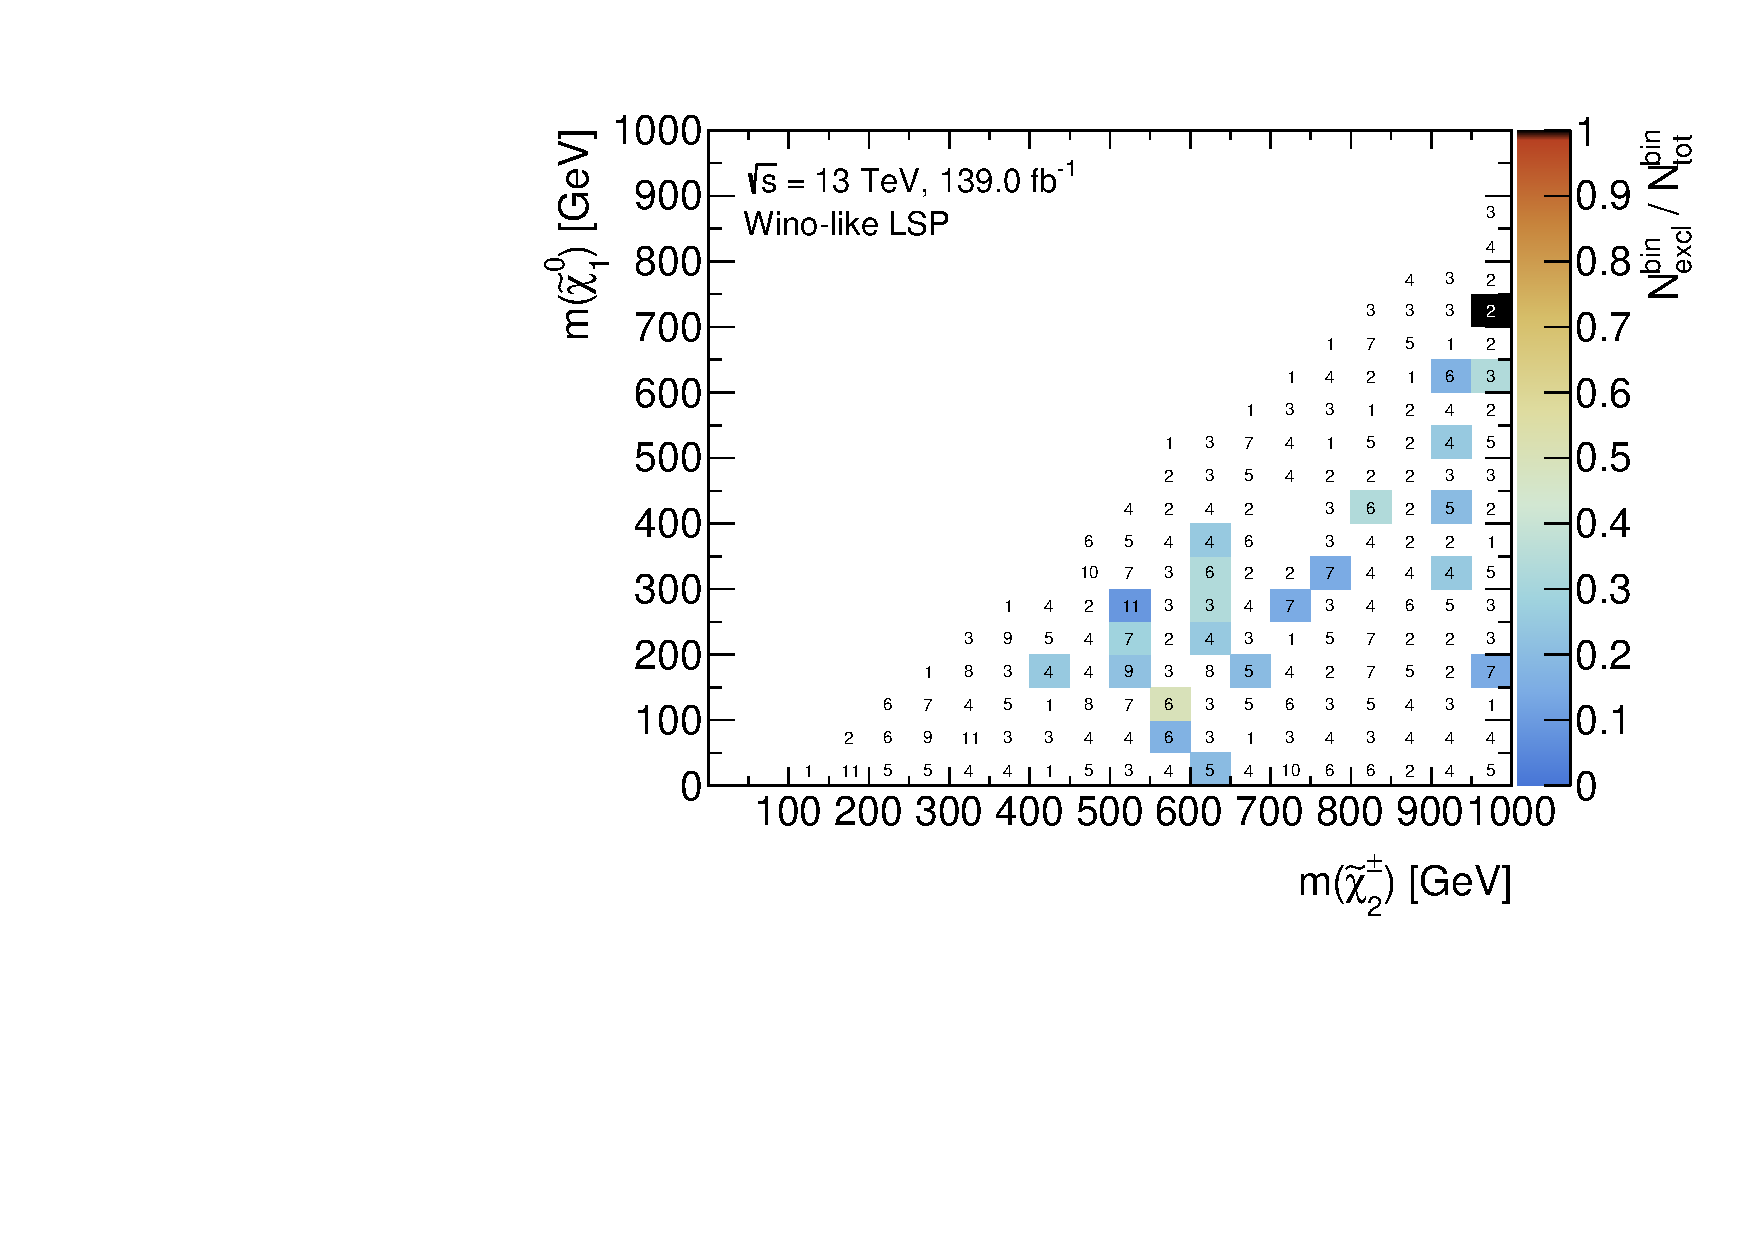
\includegraphics[width=\textwidth]{cut_wino_LSP/mchi10_mchi2p_contour}
	\end{subfigure}\hfill	
	
	\caption{Bin-by-bin fraction of excluded models as a two-dimensional function of the relevant sparticle masses. Only \gls{pmssm} models with a bino-like (wino-like) \gls{lsp} are shown on the left (right). The numbers in the bins correspond to the total number of models sampled falling into the respective bin. The number of models excluded by the \onelepton search is encoded with a colour bar ranging from 0 to 1. Where all models in a given bin are excluded, the bin is coloured in black. Bins without any models excluded are left white. Models are evaluated using the simplified likelihood of the \onelepton search. The simplified model contour is shown in orange.}
	\label{fig:impact_electroweakinos_2D_bino_lsp}
\end{figure}

% \begin{figure}
%	\centering
%	\begin{subfigure}[b]{0.5\linewidth}
%		\centering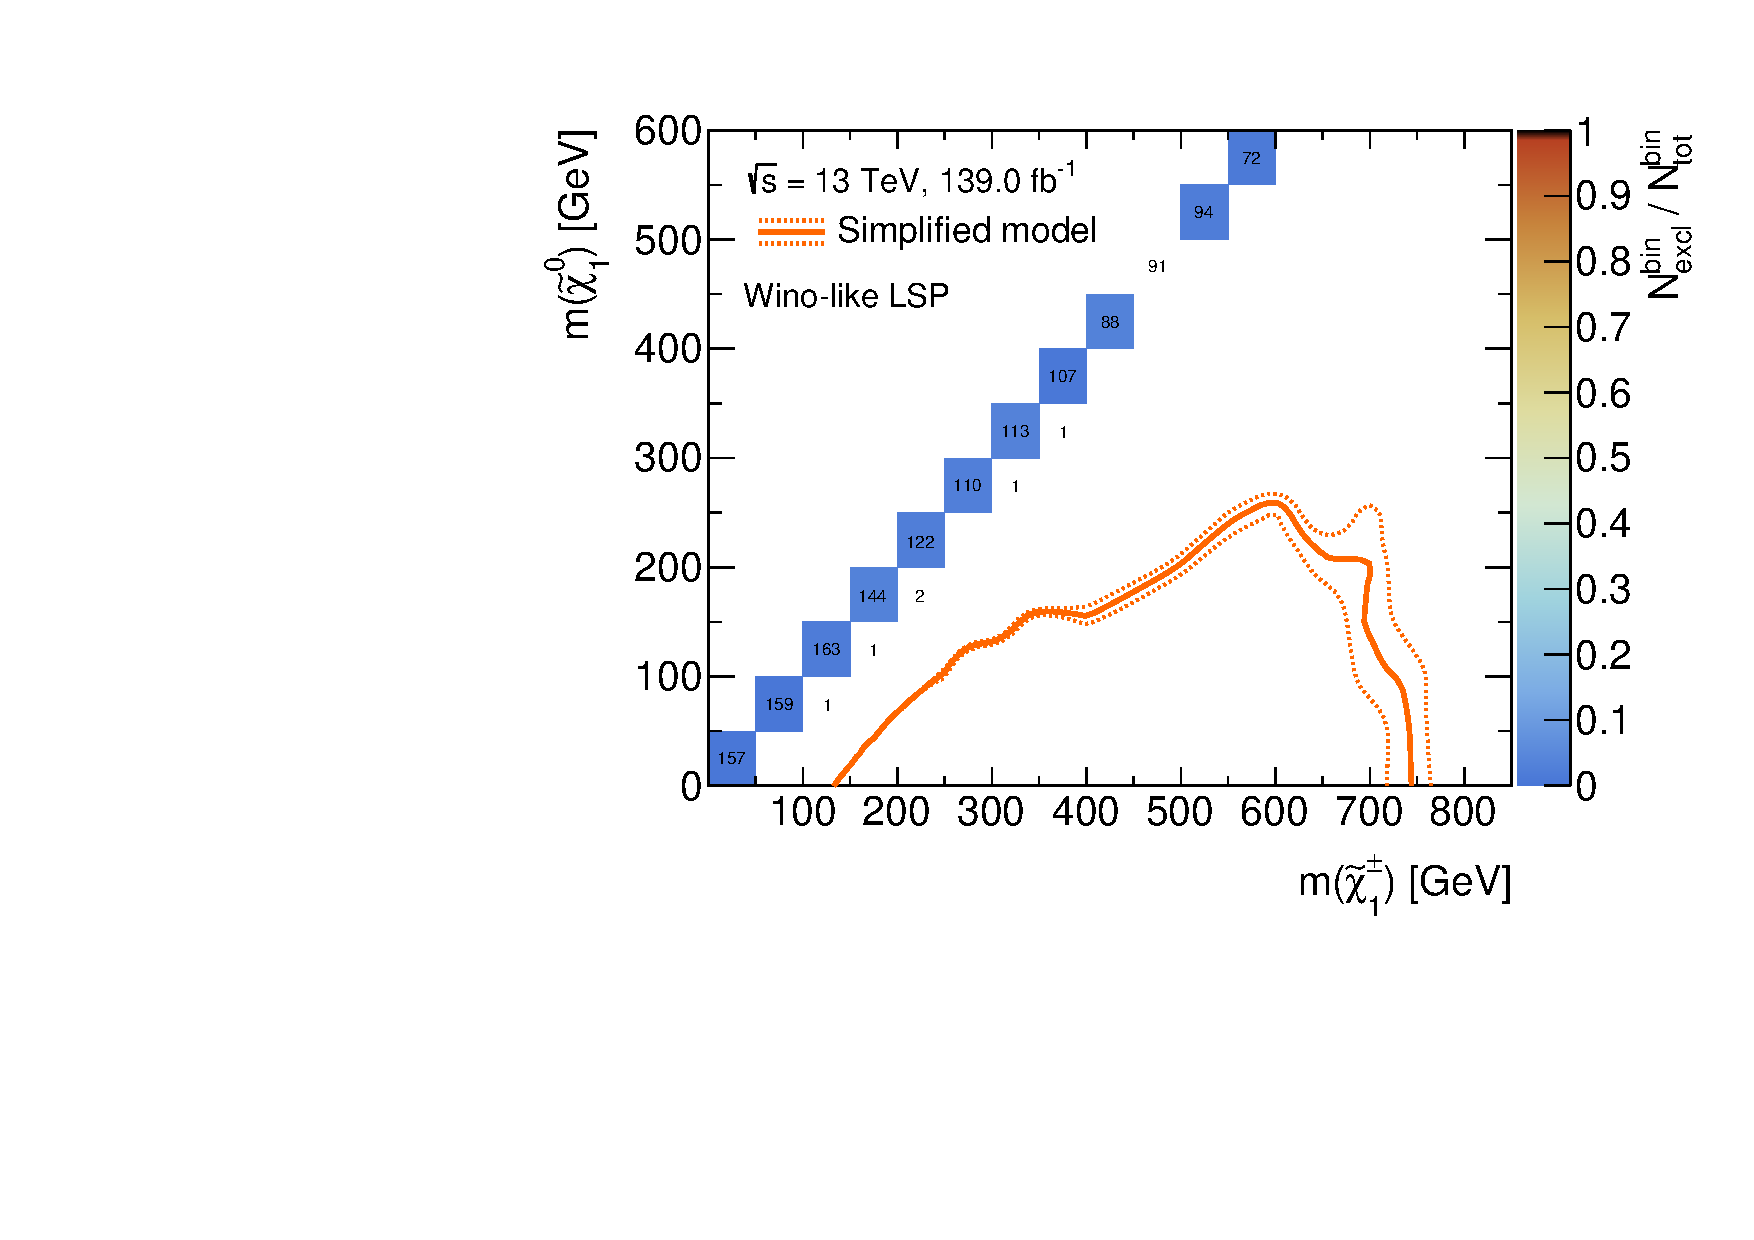
\includegraphics[width=\textwidth]{cut_wino_LSP/mchi1p_mlsp_contour}
%		\caption{\label{fig:mchi1p_mlsp_contour_wino_lsp}}
%	\end{subfigure}\hfill
%	\begin{subfigure}[b]{0.5\linewidth}
%		\centering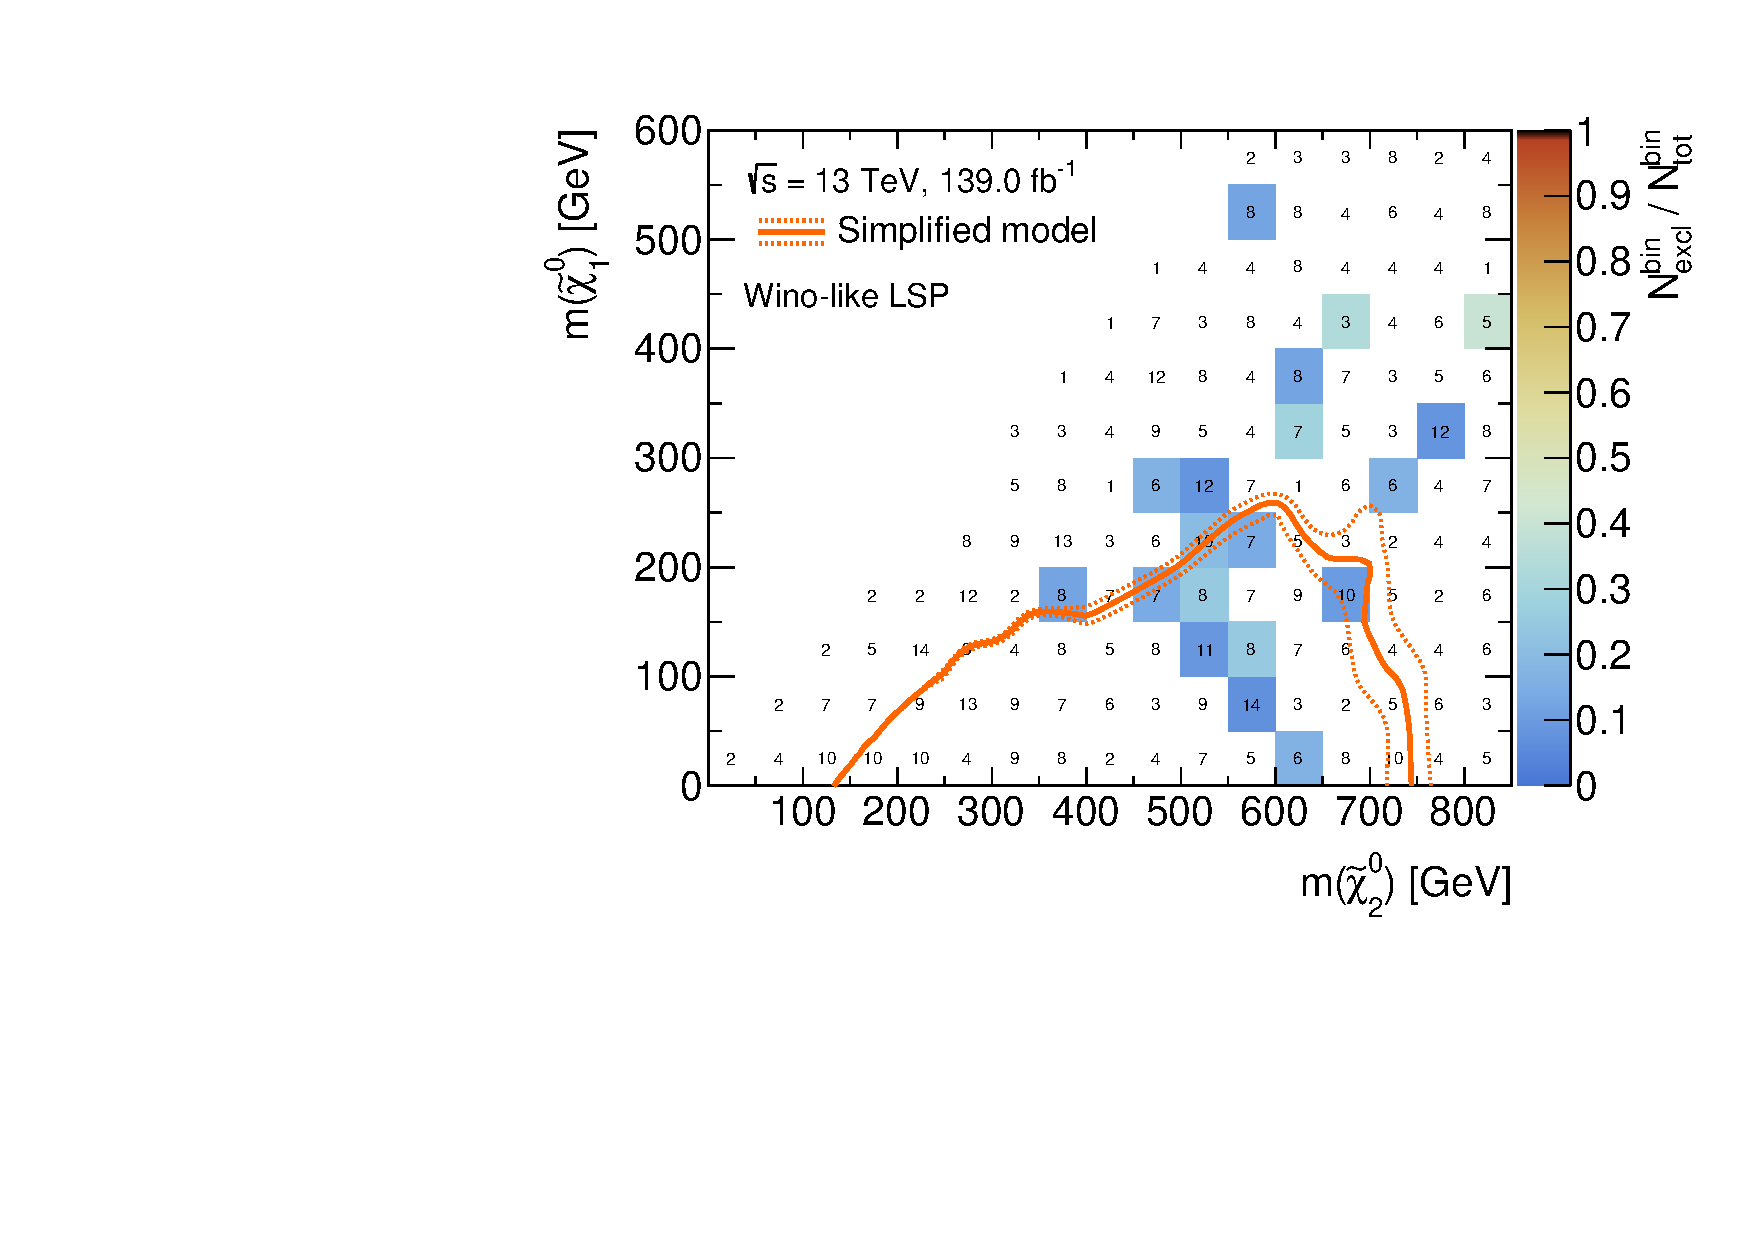
\includegraphics[width=\textwidth]{cut_wino_LSP/mchi20_mlsp_contour}
%		\caption{\label{fig:mchi20_mlsp_contour_wino_lsp}}
%	\end{subfigure}\hfill
%	\begin{subfigure}[b]{0.5\linewidth}
%		\centering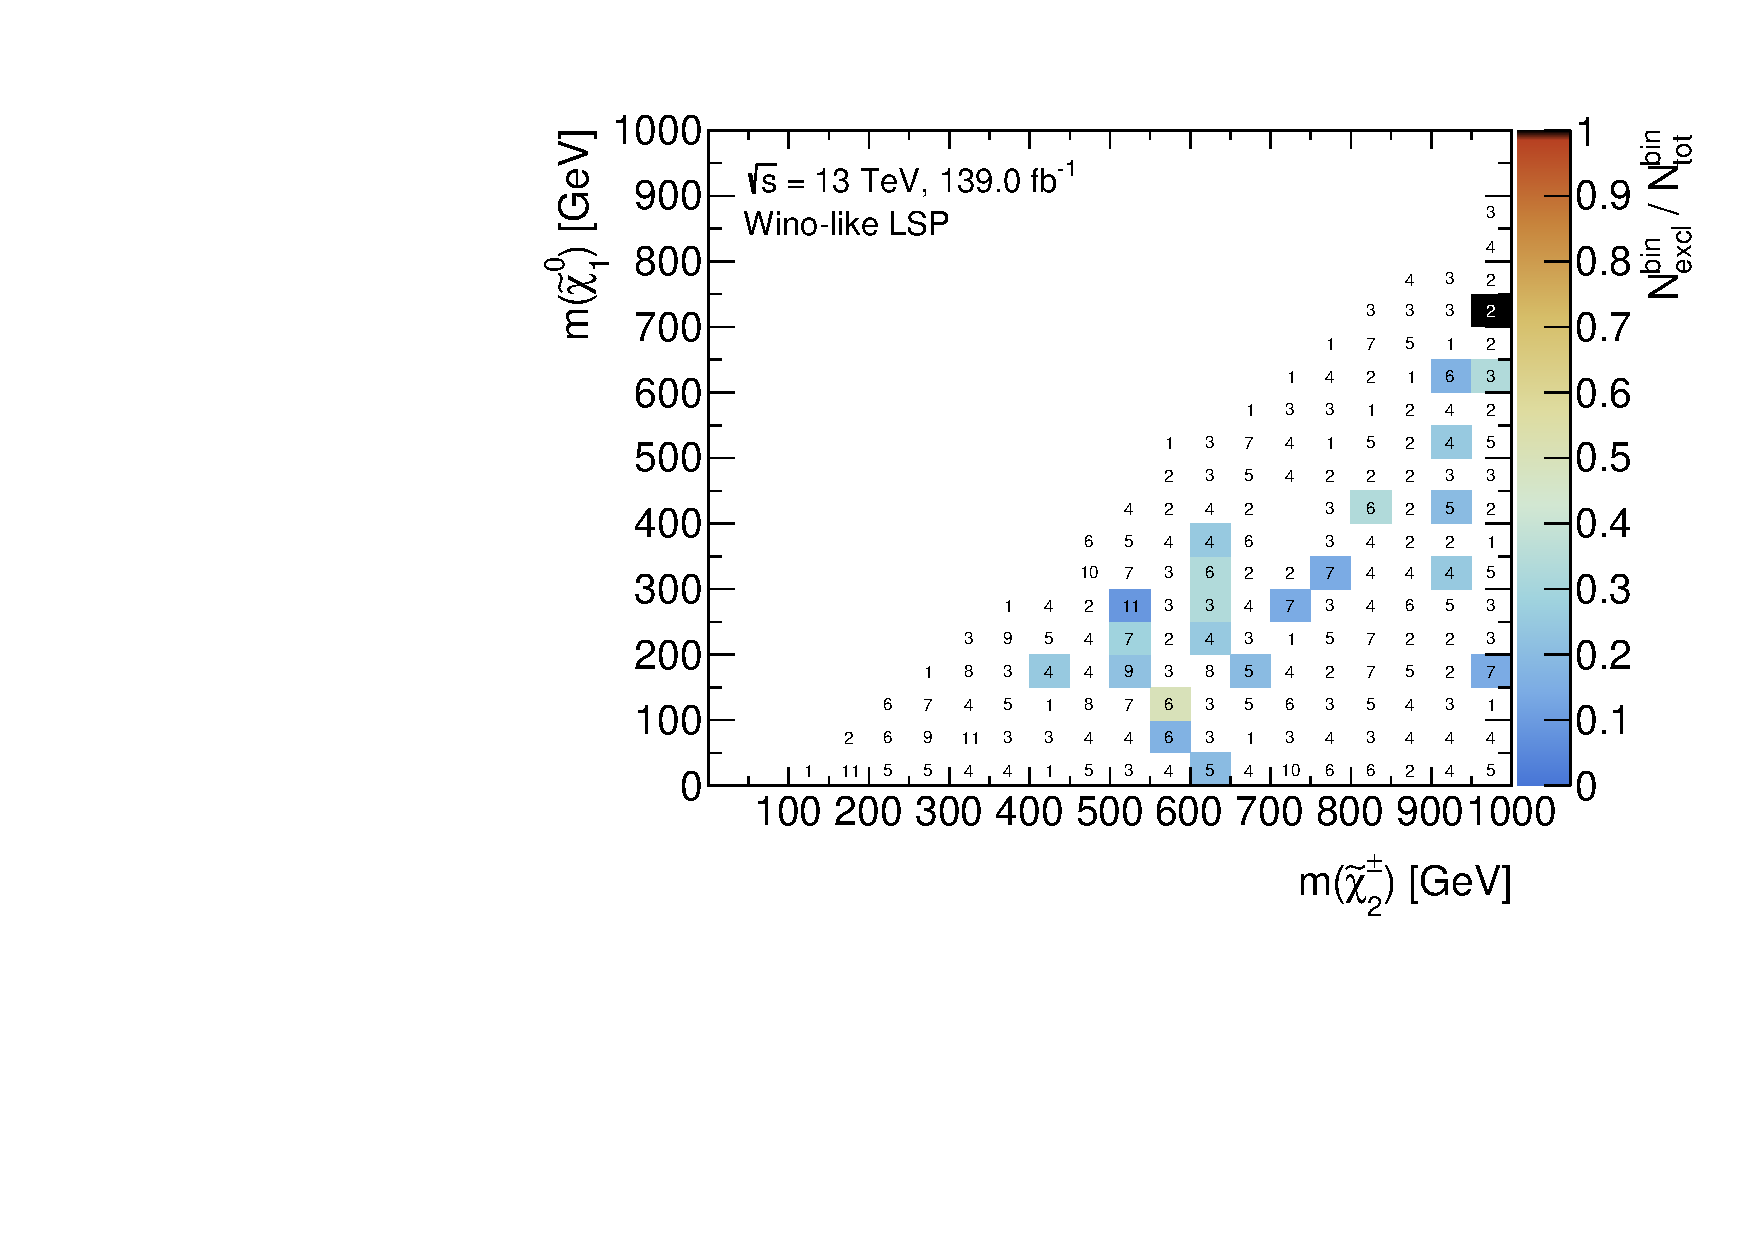
\includegraphics[width=\textwidth]{cut_wino_LSP/mchi10_mchi2p_contour}
%		\caption{\label{fig:mchi10_mchi2p_contour_wino_lsp}}
%	\end{subfigure}\hfill
%	\caption{Bin-by-bin fraction of excluded models as a function of the relevant sparticle masses. Only \gls{pmssm} models with a wino-like \gls{lsp} are shown. The numbers in the bins correspond to the total number of models sampled falling into the respective bin. The number of models excluded by the \onelepton search is encoded with a colour bar ranging from 0 to 1. Where all models in a given bin are excluded, the bin is coloured in black. Bins without a models excluded are left white. Models are evaluated using the simplified likelihood of the \onelepton search. The simplified model contour is shown in orange.}
%	\label{fig:impact_electroweakinos_2D_wino_lsp}
%\end{figure}

% \begin{figure}
%	\centering
%	\begin{subfigure}[b]{0.5\linewidth}
%		\centering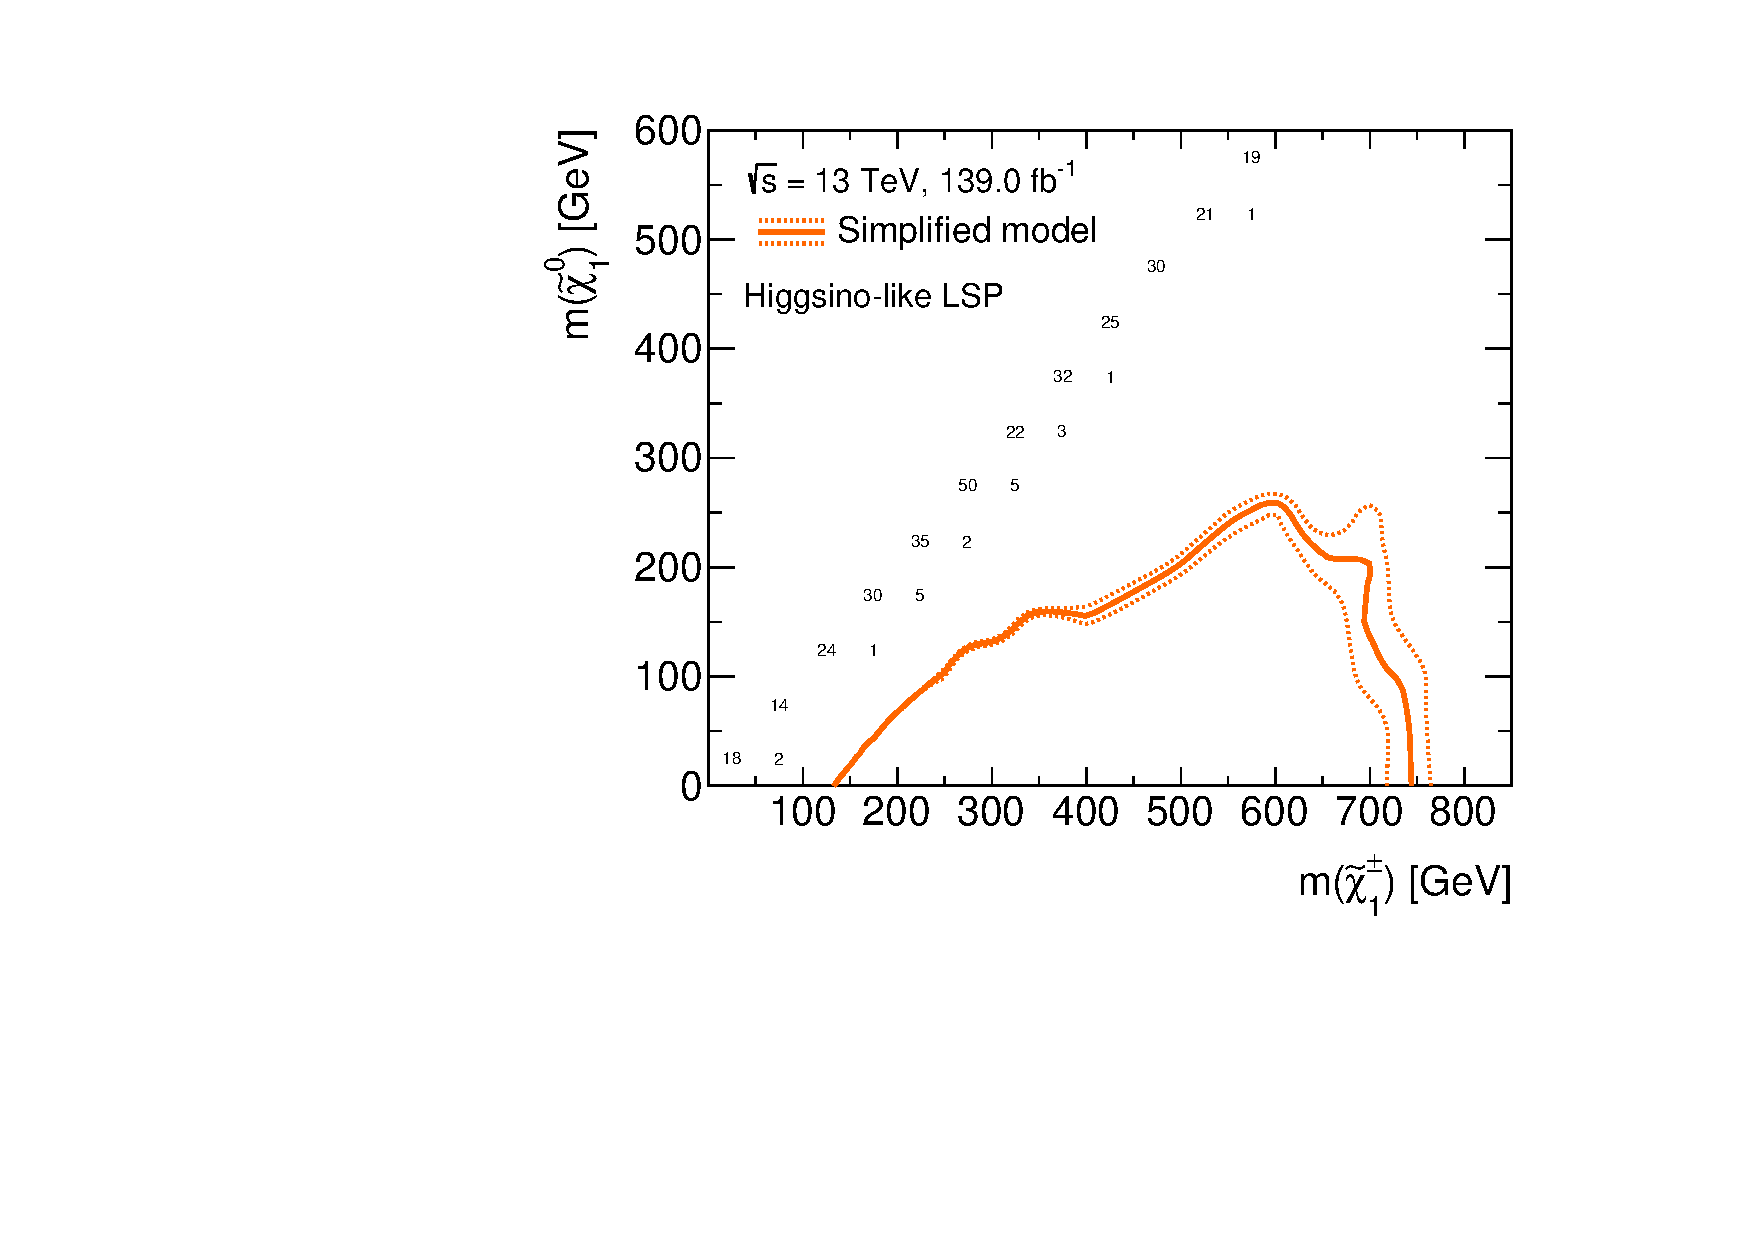
\includegraphics[width=\textwidth]{cut_higgsino_LSP/mchi1p_mlsp_contour}
%		\caption{\label{fig:mchi1p_mlsp_contour_higgsino_lsp}}
%	\end{subfigure}\hfill
%	\begin{subfigure}[b]{0.5\linewidth}
%		\centering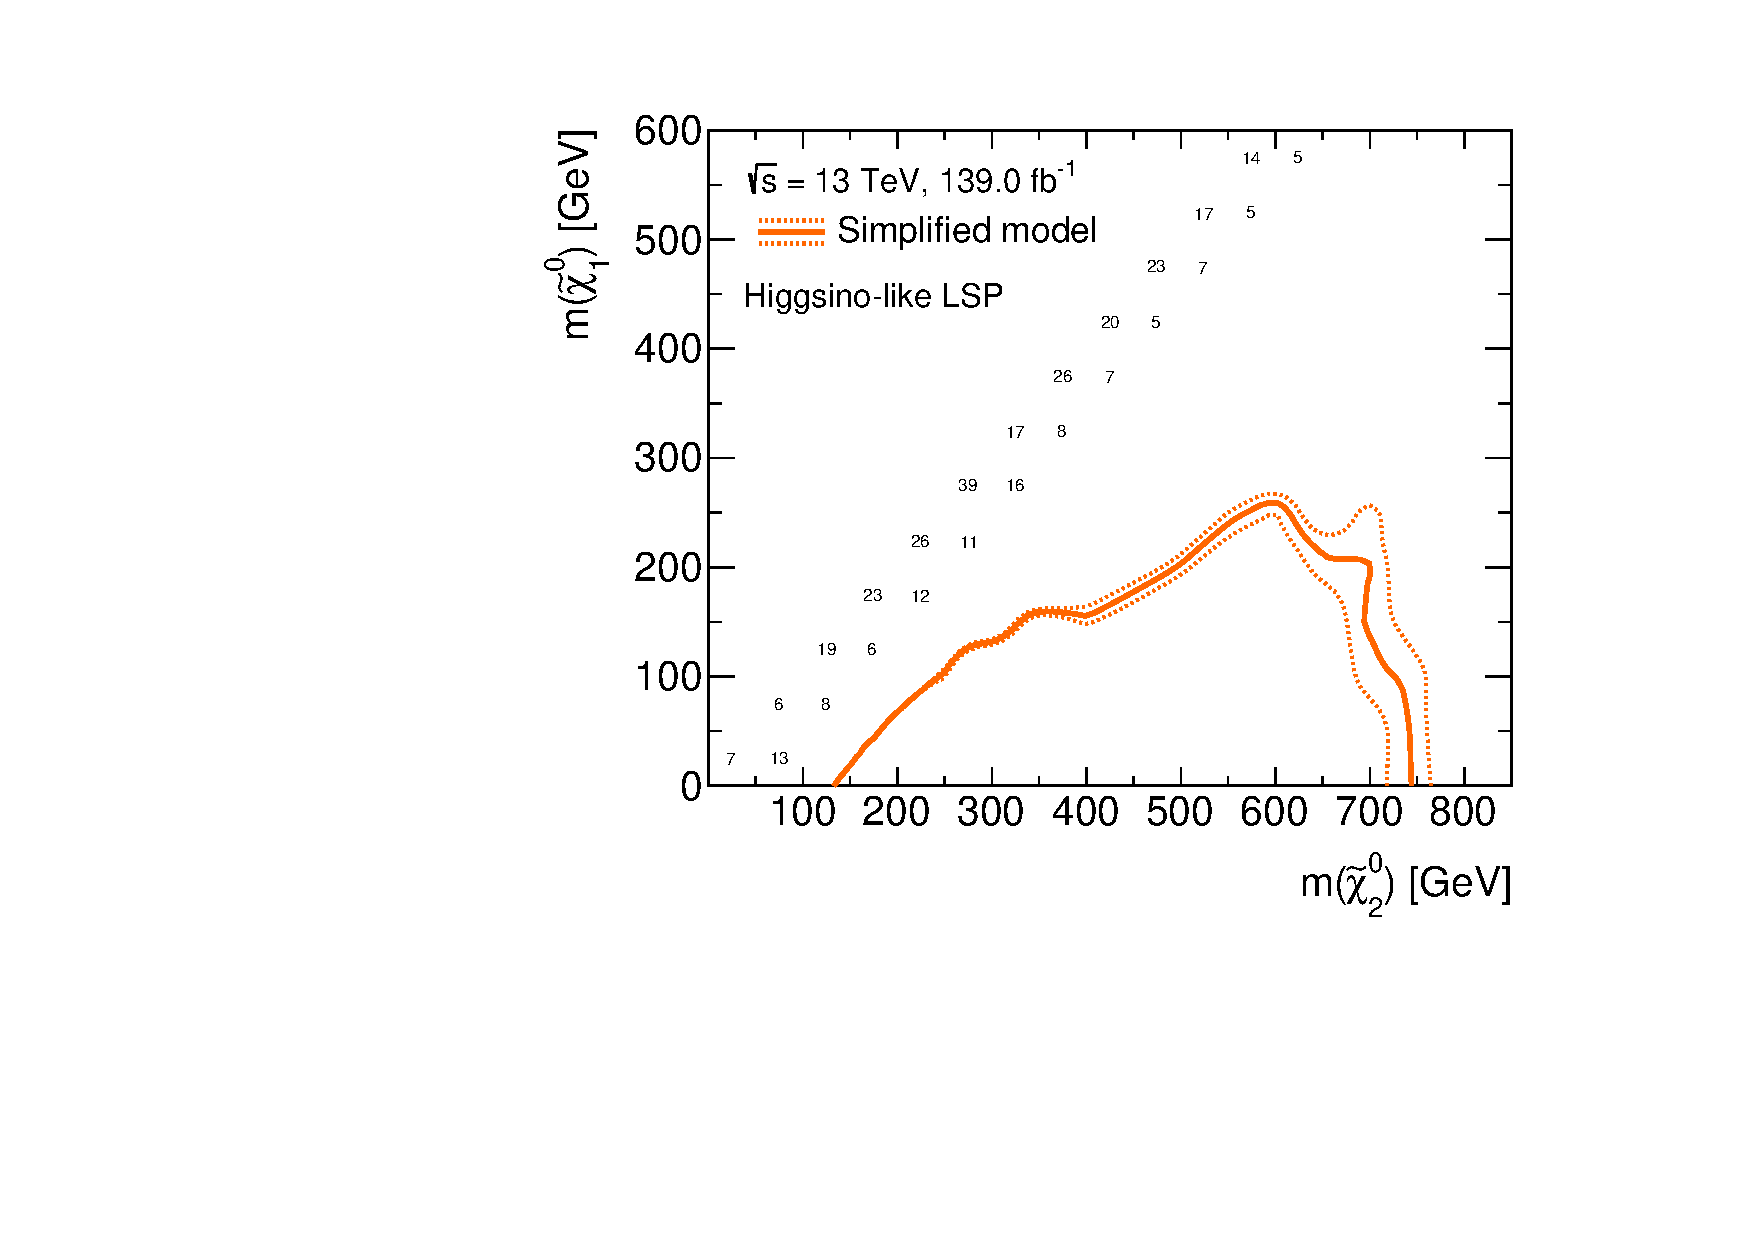
\includegraphics[width=\textwidth]{cut_higgsino_LSP/mchi20_mlsp_contour}
%		\caption{\label{fig:mchi20_mlsp_contour_higgsino_lsp}}
%	\end{subfigure}\hfill
%	\begin{subfigure}[b]{0.5\linewidth}
%		\centering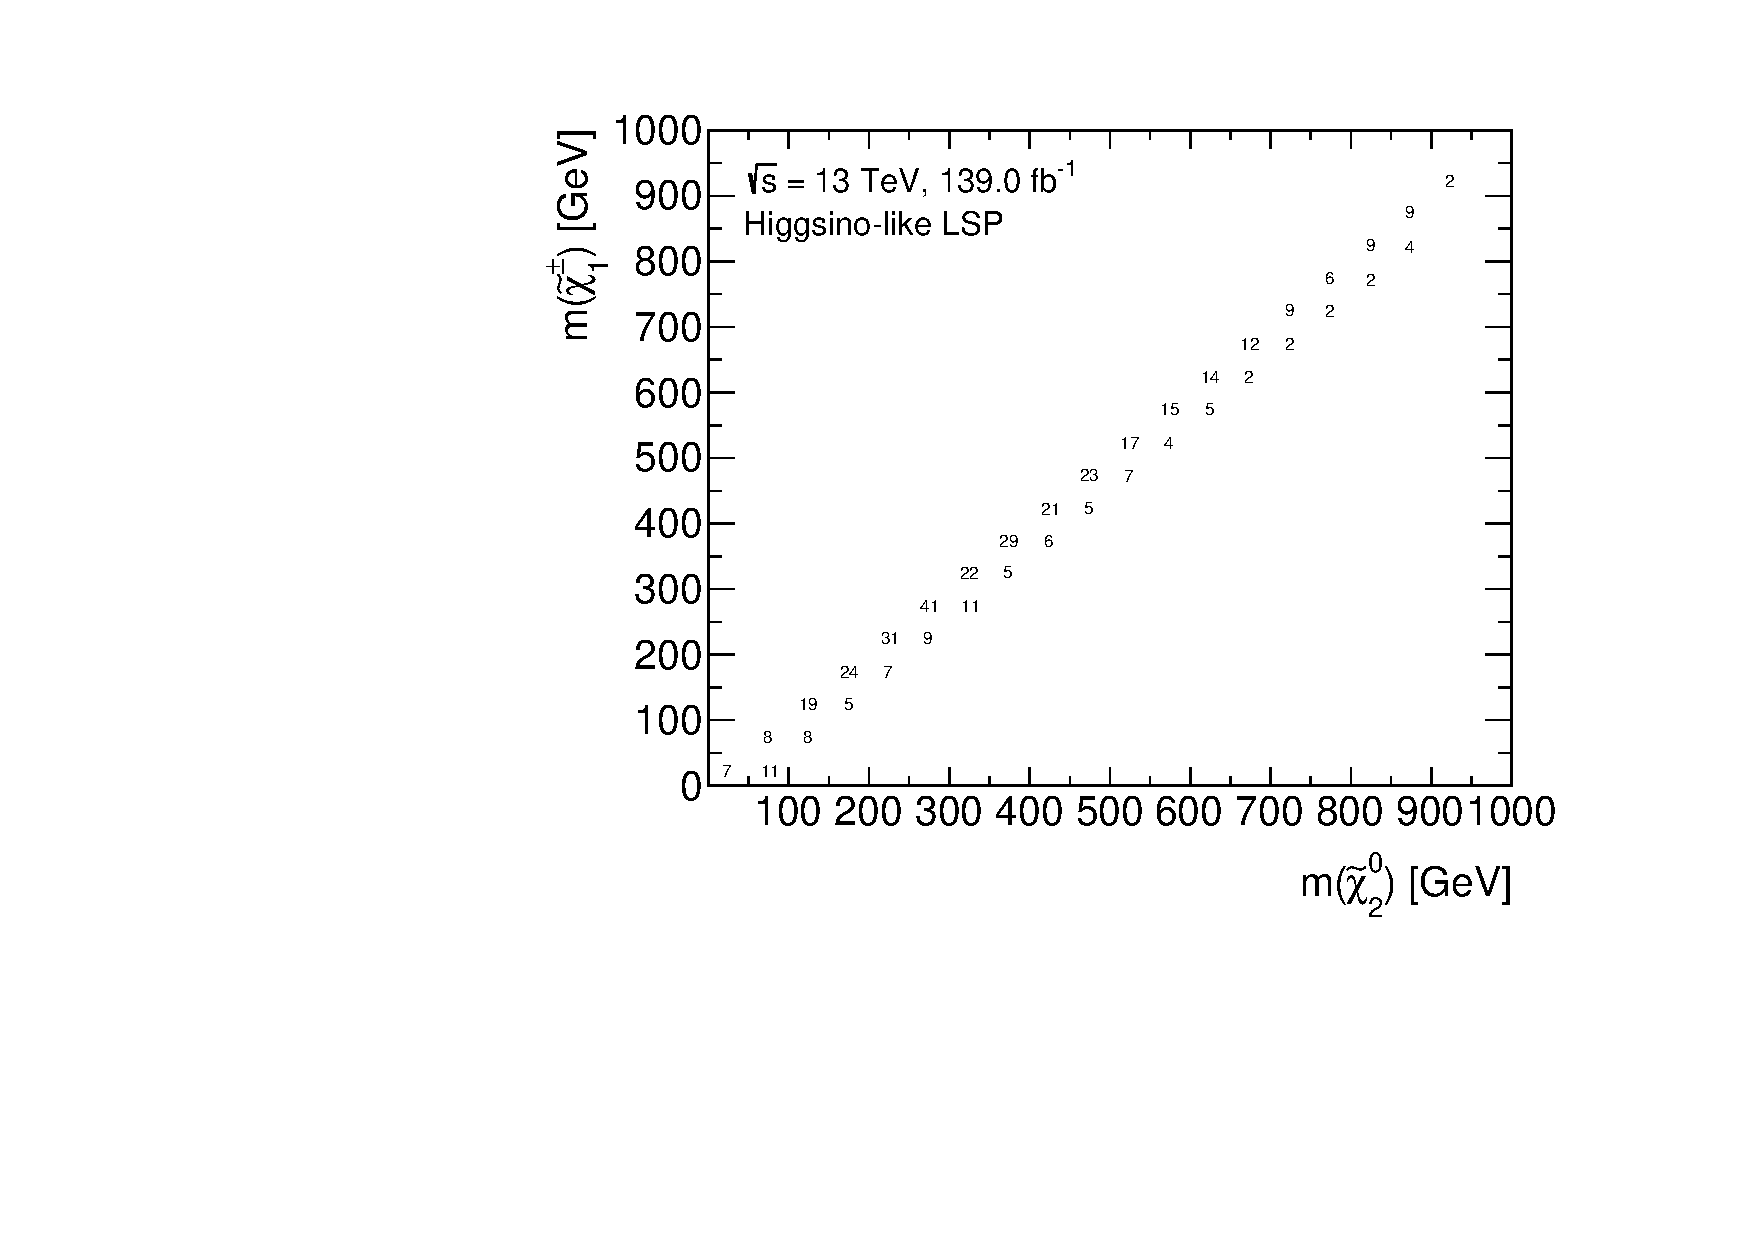
\includegraphics[width=\textwidth]{cut_higgsino_LSP/mchi1p_mchi20_contour}
%		\caption{\label{fig:mchi1p_mchi20_contour_higgsino_lsp}}
%	\end{subfigure}\hfill
%	\caption{Bin-by-bin fraction of excluded models as a function of the relevant sparticle masses. Only \gls{pmssm} models with a higgsino-like \gls{lsp} are shown. The numbers in the bins correspond to the total number of models sampled falling into the respective bin. The number of models excluded by the \onelepton search is encoded with a colour bar ranging from 0 to 1. Where all models in a given bin are excluded, the bin is coloured in black. Bins without a models excluded are left white. Models are evaluated using the simplified likelihood of the \onelepton search. The simplified model contour is shown in orange.}
%	\label{fig:impact_electroweakinos_2D_higgsino_lsp}
%\end{figure}


\FloatBarrier


\section{Impact on electroweakinos}

As illustrated in \cref{fig:higgs_coupling_neutralino}, the couplings of the $\neutr$ to the Higgs boson are suppressed by powers of $\vert\mu\vert/M_2$ in the wino-like and bino-like scenarios~\cite{Arbey:2012fa}, meaning that the branching fraction of $\neutr \rightarrow h \lsp$ takes on reasonably high values only in models with an \gls{lsp} that is nearly pure bino.

\Cref{fig:higgsino_spectrum} shows the compressed mass spectrum of an exemplary \gls{pmssm} model point with higgsino-like $\lsp$, a model that the \onelepton search is not expected to be sensitive to.

\begin{figure}[h]
	\centering
	\begin{subfigure}[b]{0.49\linewidth}
		\centering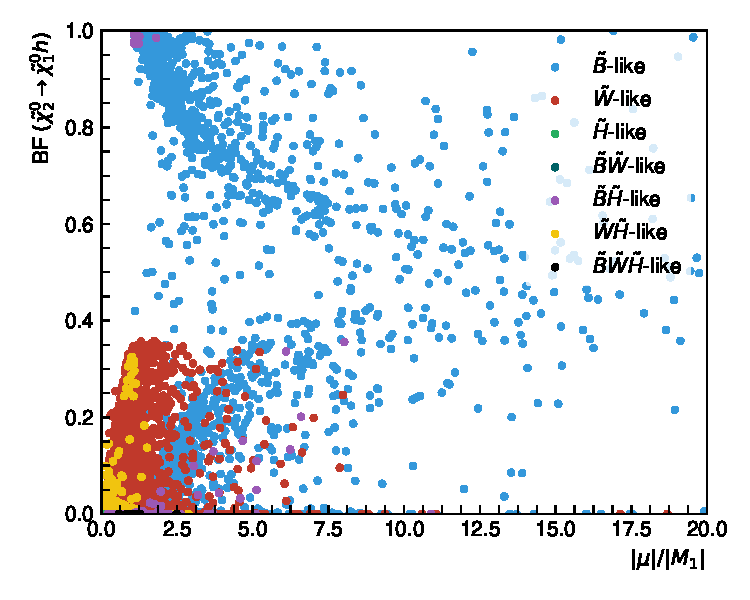
\includegraphics[width=\textwidth]{scatter/lsp_types_BR_Higgs_muM1}
		\caption{\label{fig:lsp_types_BR_Higgs_muM1}}
	\end{subfigure}\hfill
	\begin{subfigure}[b]{0.49\linewidth}
		\centering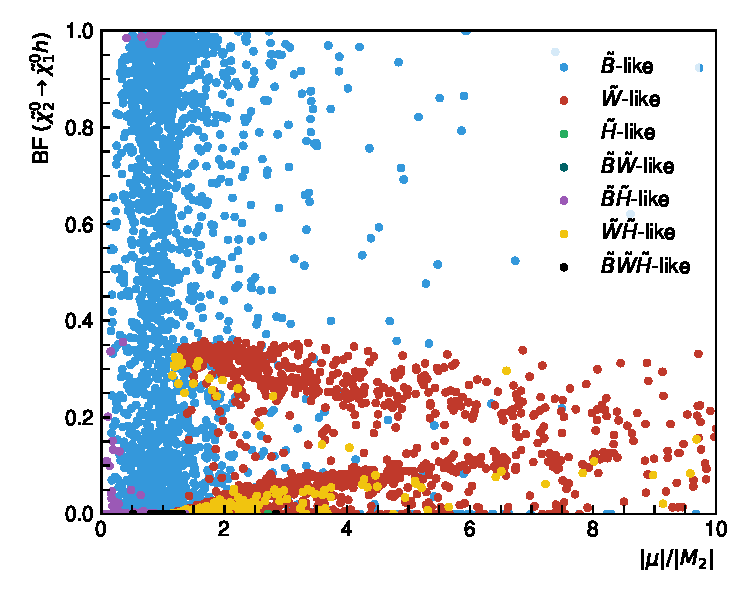
\includegraphics[width=\textwidth]{scatter/lsp_types_BR_Higgs_muM2}
		\caption{\label{fig:lsp_types_BR_Higgs_muM2}}
	\end{subfigure}\hfill
	\caption{Density of the \gls{pmssm} models projected onto the plane spanned by $\mathrm{BF}(\neutr \rightarrow h \lsp)$ and \subref{fig:lsp_types_BR_Higgs_muM1} $\vert\mu\vert/\vert M_1 \vert$ or \subref{fig:lsp_types_BR_Higgs_muM2} $\vert\mu\vert/\vert M_2 \vert$. Models are shown as a function of their $\lsp$ type.}
	\label{fig:higgs_coupling_neutralino}
\end{figure}

\begin{figure}[h]
\floatbox[{\capbeside\thisfloatsetup{capbesideposition={right,center},capbesidewidth=0.50\textwidth}}]{figure}[\FBwidth]
{\caption{Mass spectrum of an exemplary \gls{pmssm} model with a higgsino-like $\lsp$. The branching fractions of the different decays are indicated through the width and and greyscale colour (pure black being 100\%, pure white being 0\%) of the arrows. Branching fractions below 10\% are suppressed for the sake of visibility. Figure generated using \texttt{pyslha}~\cite{pyslha:2013jua}.}\label{fig:higgsino_spectrum}}
{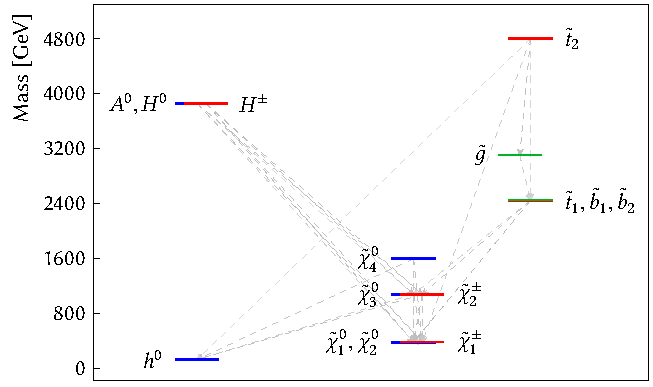
\includegraphics[width=0.50\textwidth]{thesis_plot_6898.pdf}}
\end{figure}

\FloatBarrier

\section{Impact on pMSSM parameters}

In \cref{fig:impact_pMSSM_parameters_1D_2}, the impact of the \onelepton search on the reminaing \gls{pmssm} parameters sampled, not already shown in \cref{sec:impact_pmssm_parameters}, are provided. As before, the full set of models evaluated with the \onelepton search is shown as black line, while the bin-wise number of models excluded by the search are indicated with the blue histogram. An additional pad indicates the fraction of models excluded in each bin.

\begin{figure}
	\centering
	\begin{subfigure}[b]{0.4\linewidth}
		\centering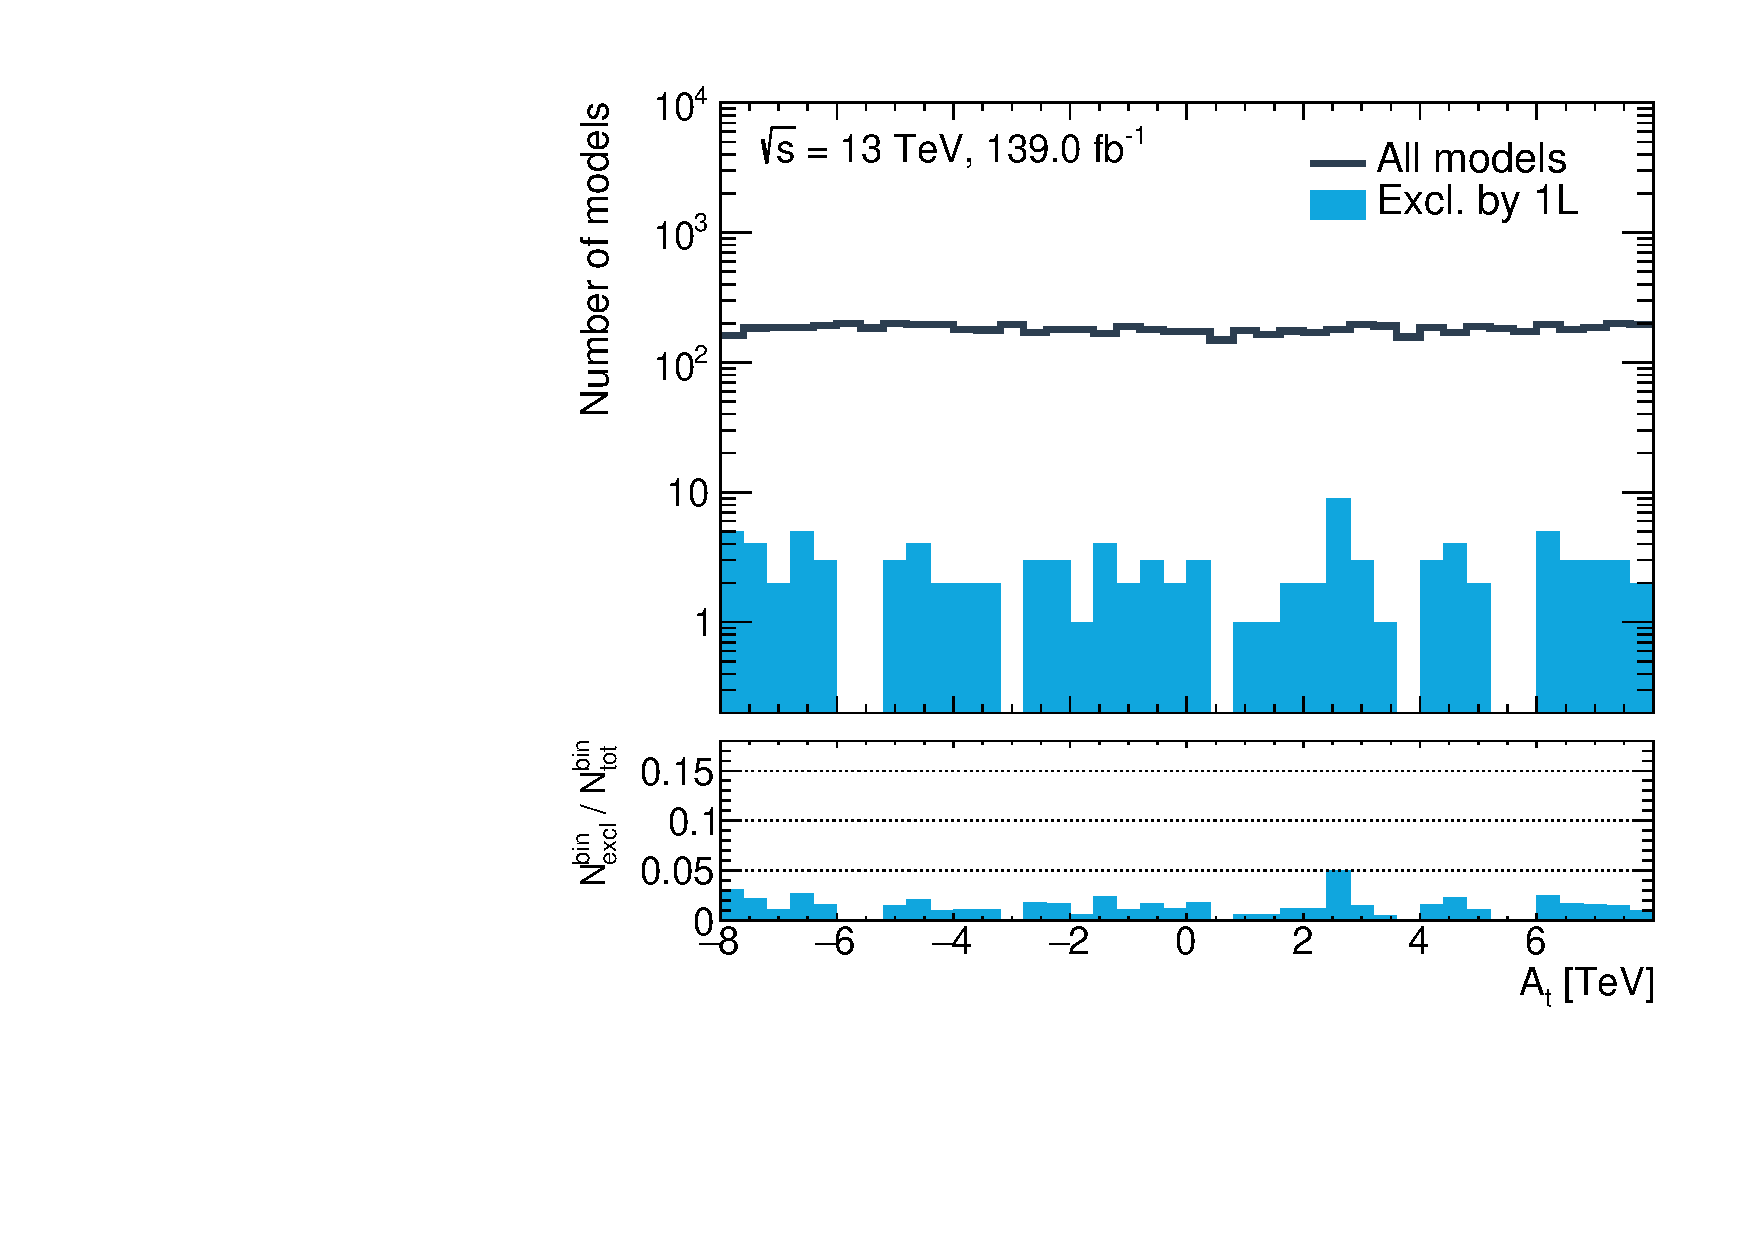
\includegraphics[width=\textwidth]{1D/At}
	\end{subfigure}
	\begin{subfigure}[b]{0.4\linewidth}
		\centering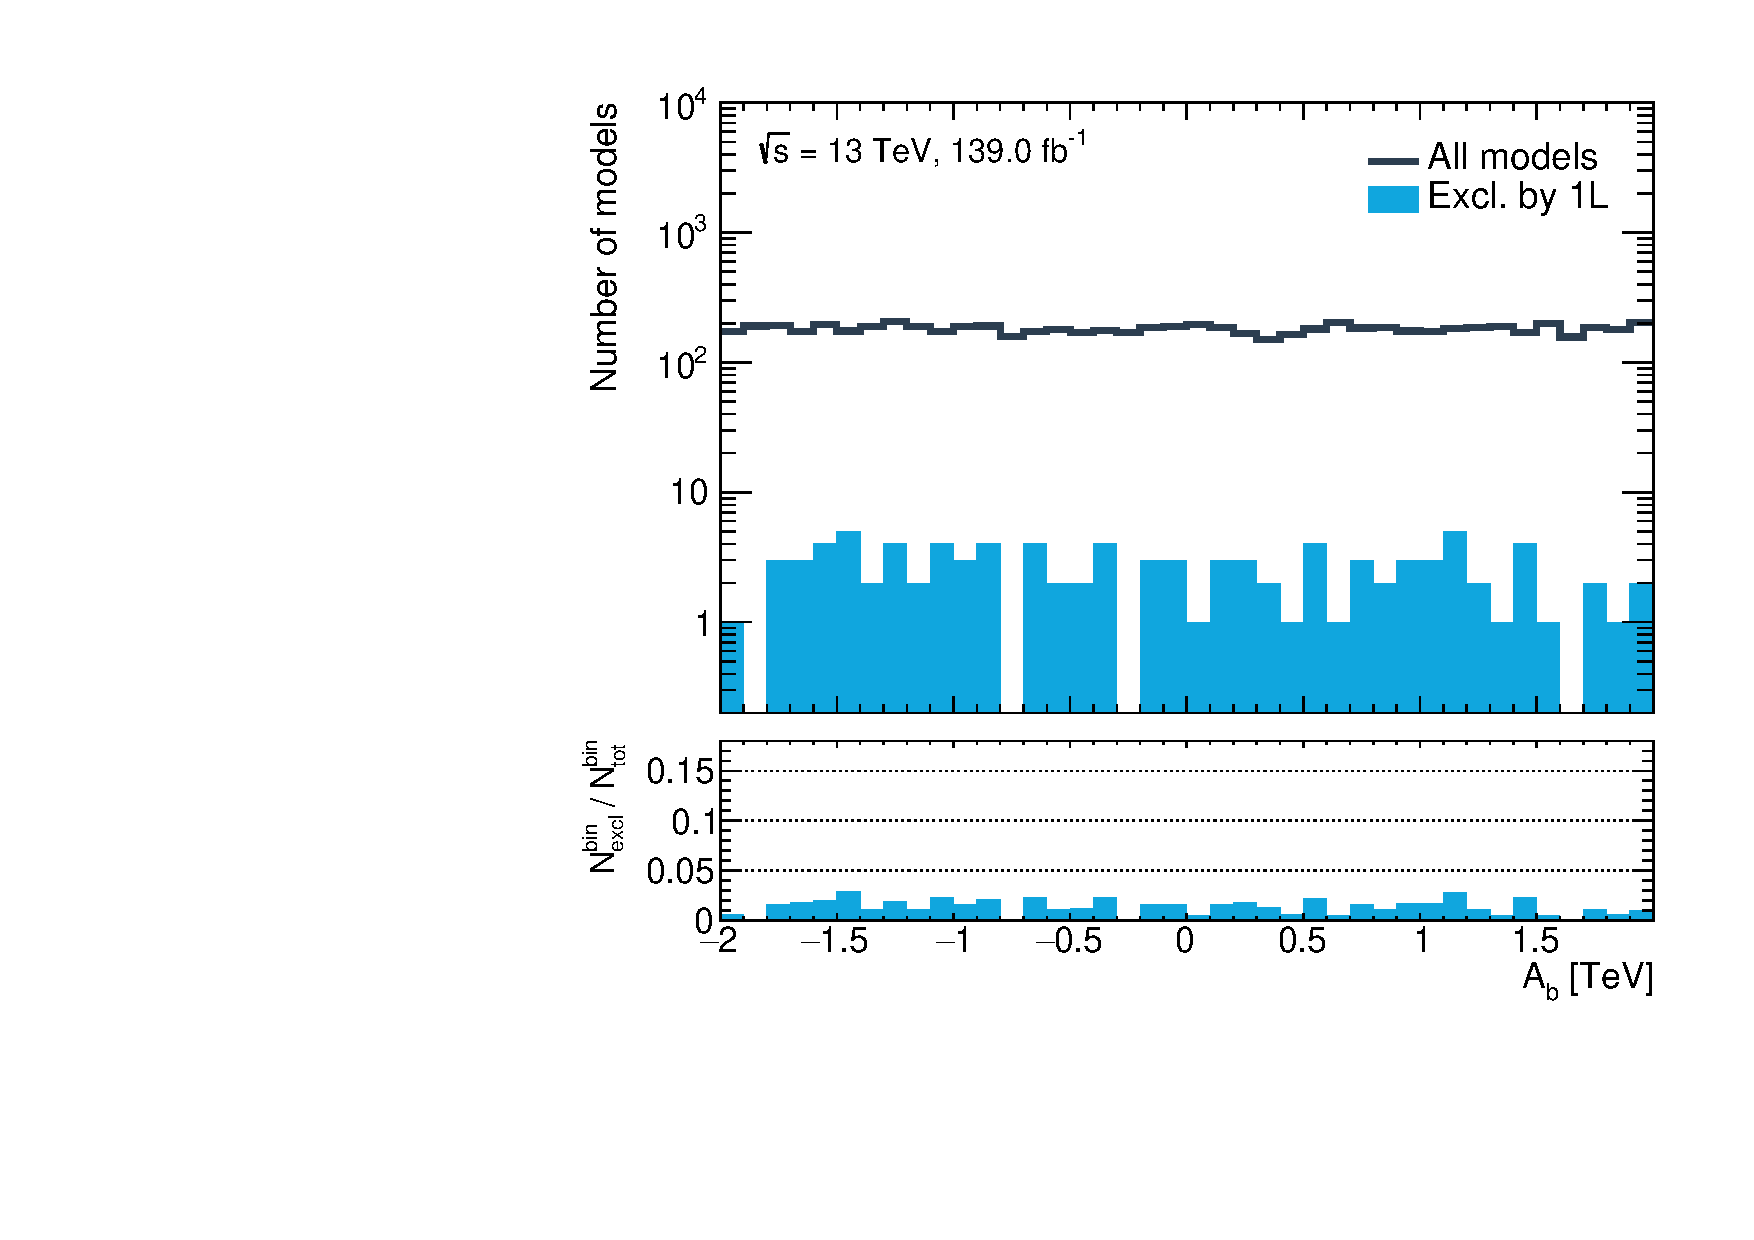
\includegraphics[width=\textwidth]{1D/Ab}
	\end{subfigure}
	\begin{subfigure}[b]{0.4\linewidth}
		\centering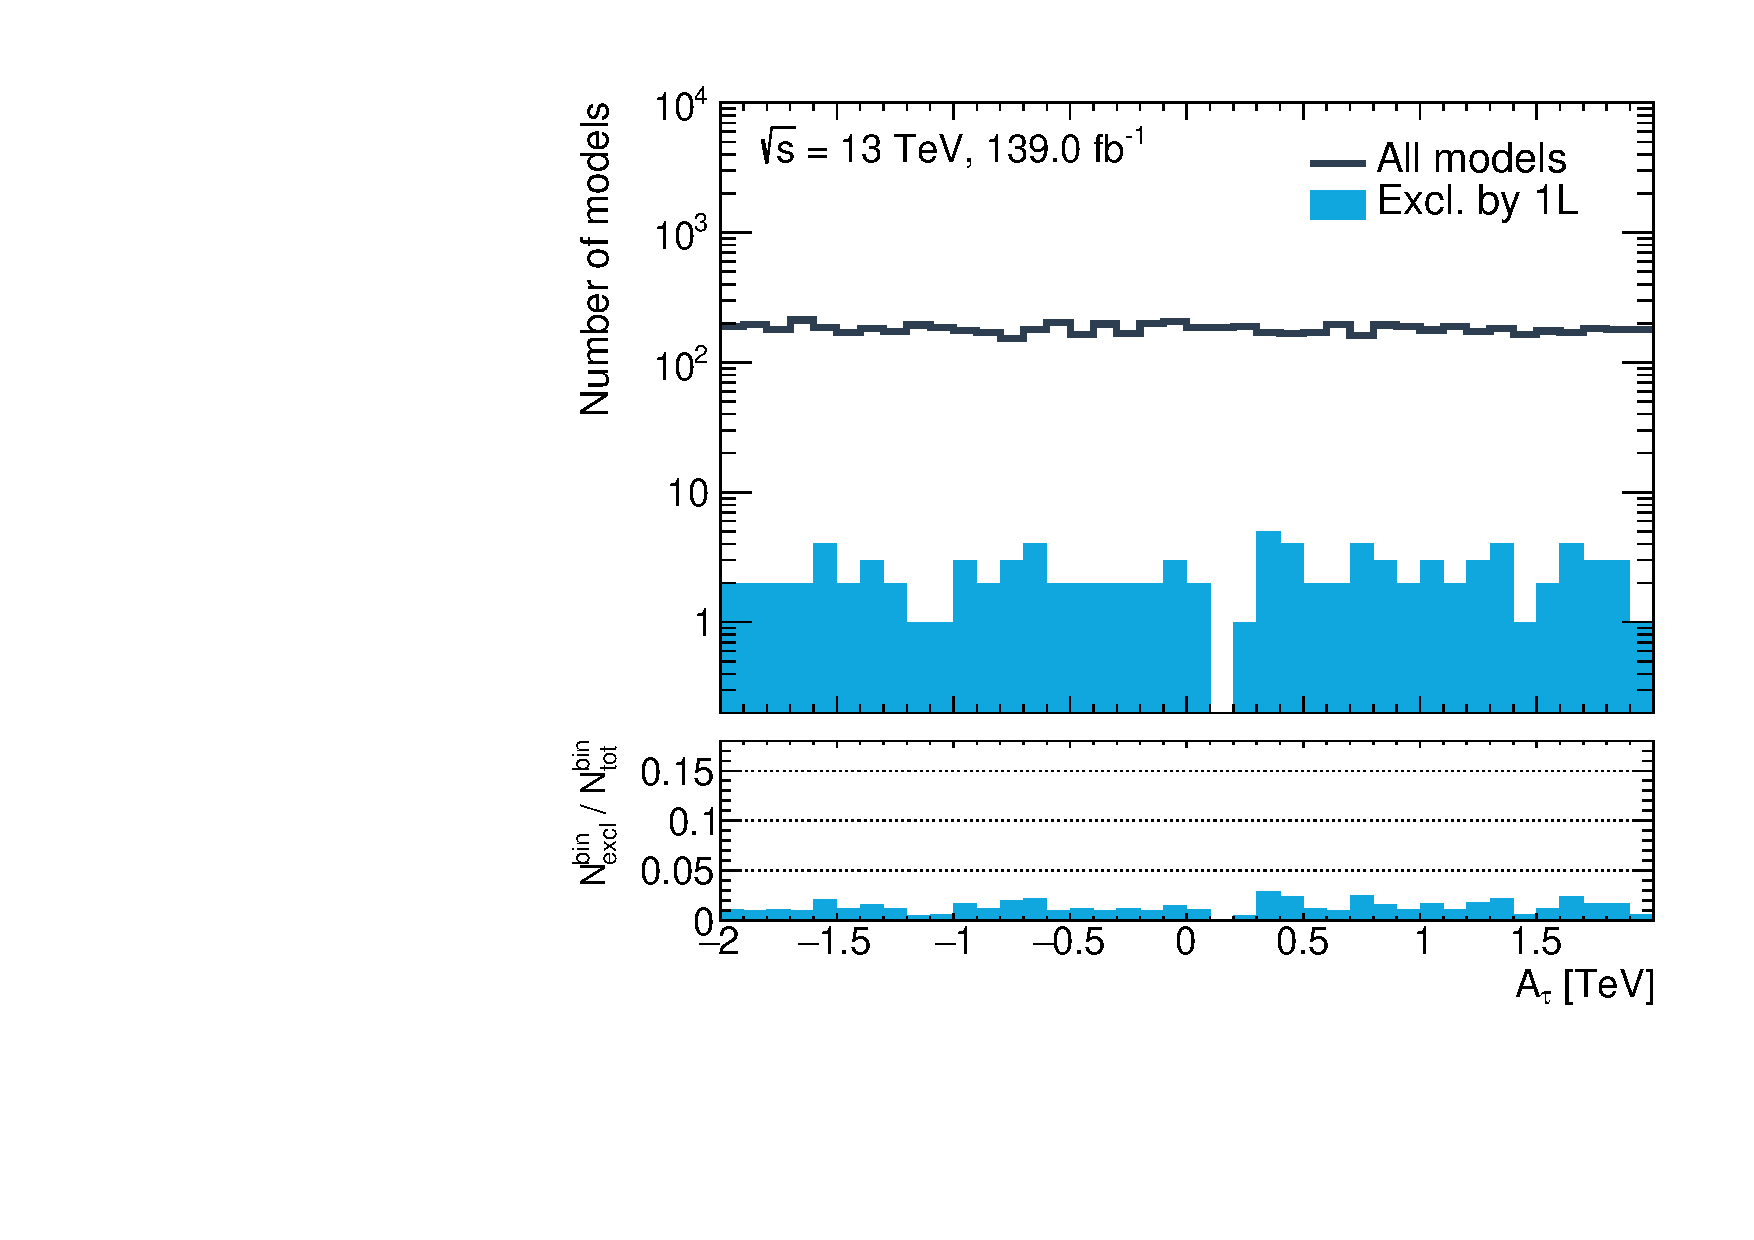
\includegraphics[width=\textwidth]{1D/Atau}
	\end{subfigure}
	\begin{subfigure}[b]{0.4\linewidth}
		\centering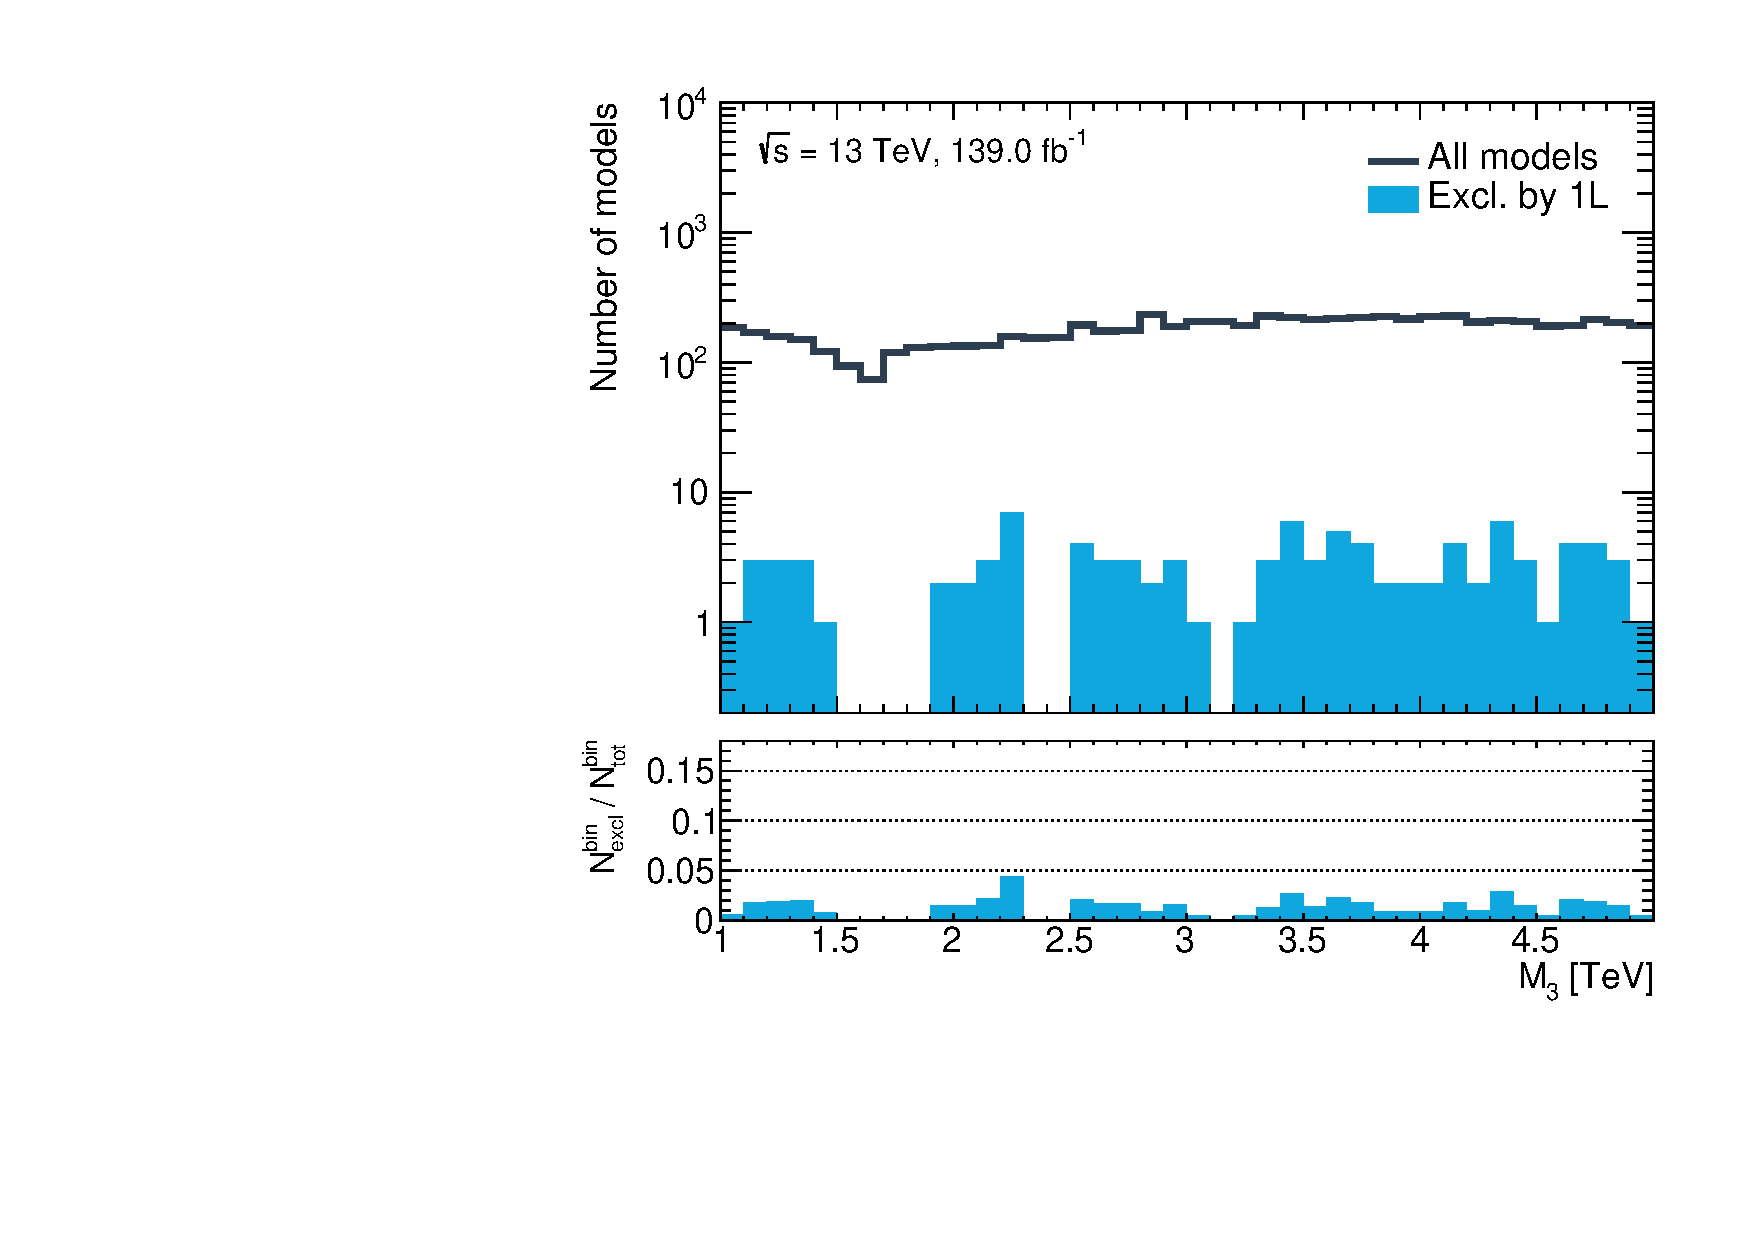
\includegraphics[width=\textwidth]{1D/M3}
	\end{subfigure}
	\begin{subfigure}[b]{0.4\linewidth}
		\centering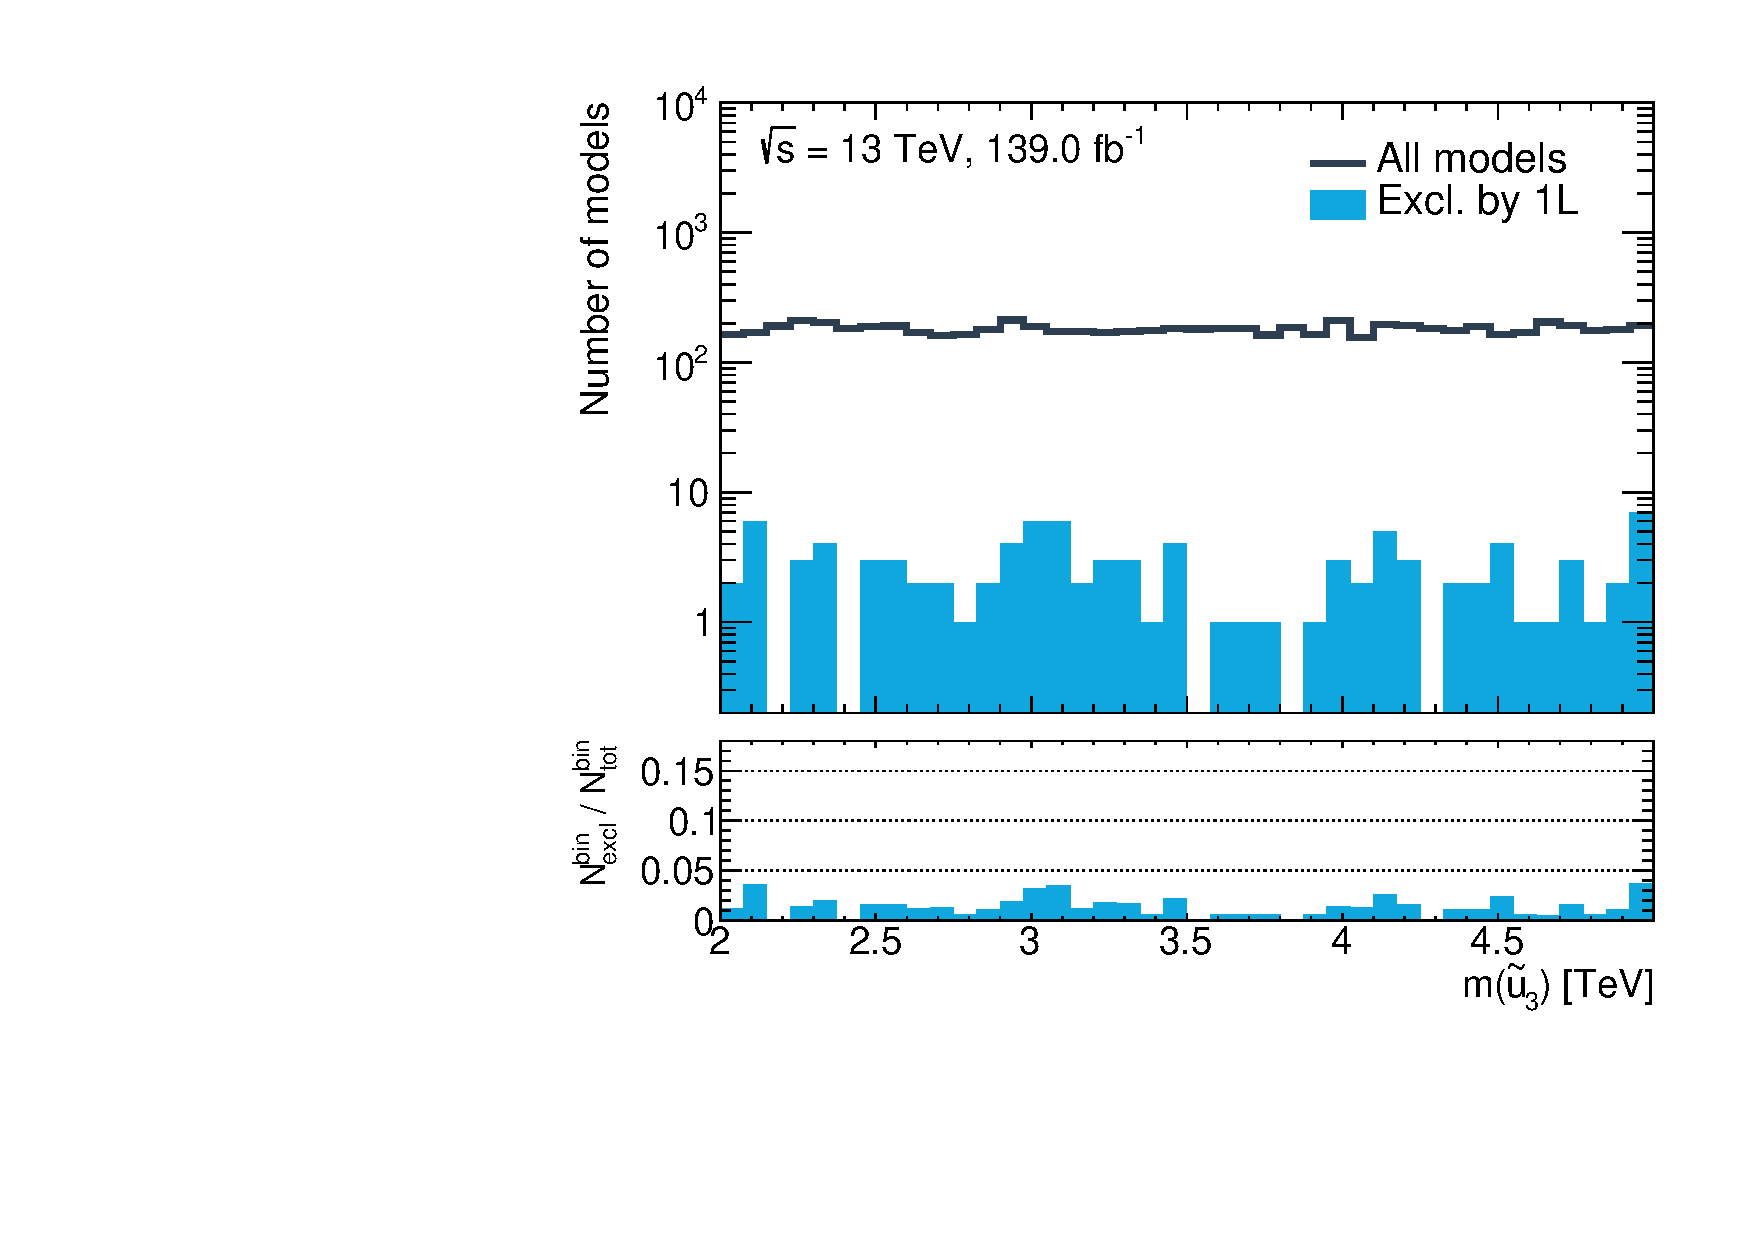
\includegraphics[width=\textwidth]{1D/mtR}
	\end{subfigure}
	\begin{subfigure}[b]{0.4\linewidth}
		\centering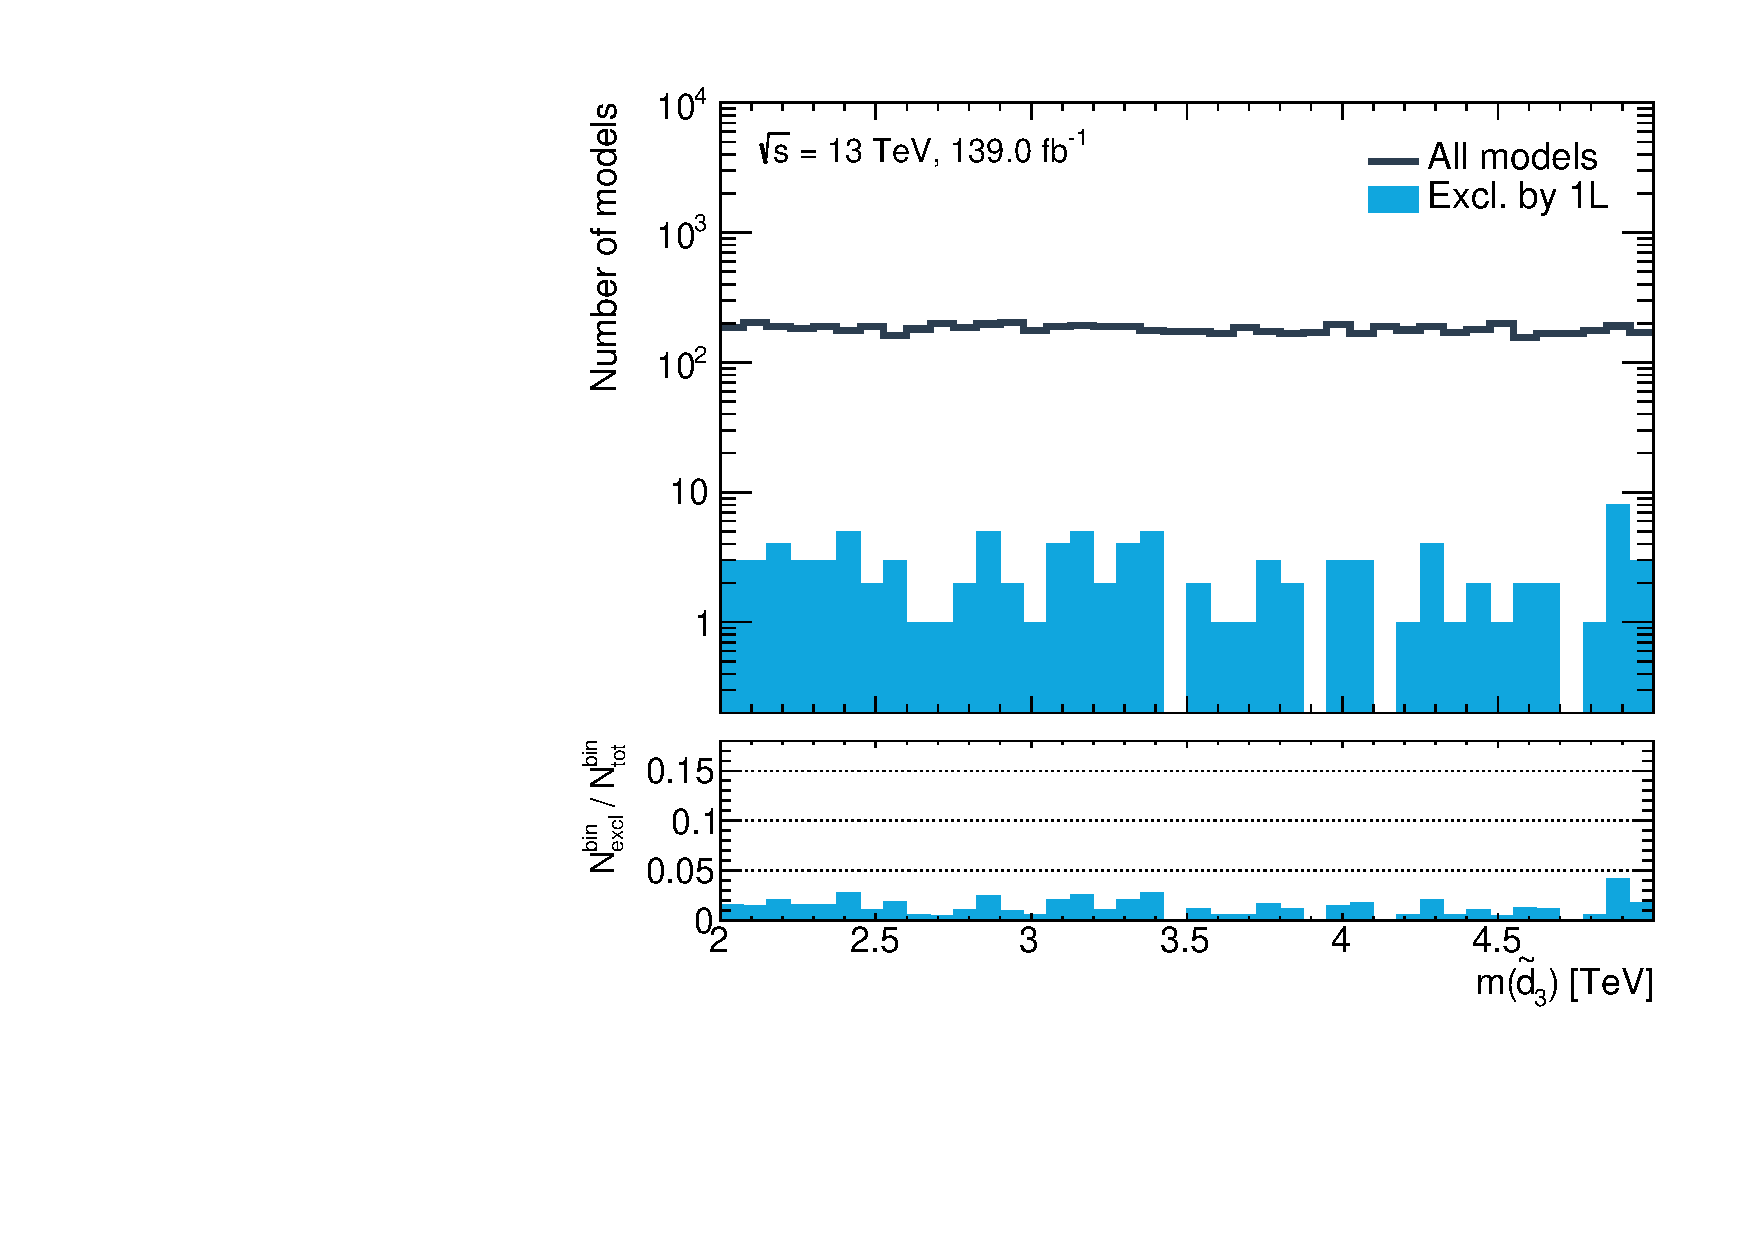
\includegraphics[width=\textwidth]{1D/mbR}
	\end{subfigure}
	\begin{subfigure}[b]{0.4\linewidth}
		\centering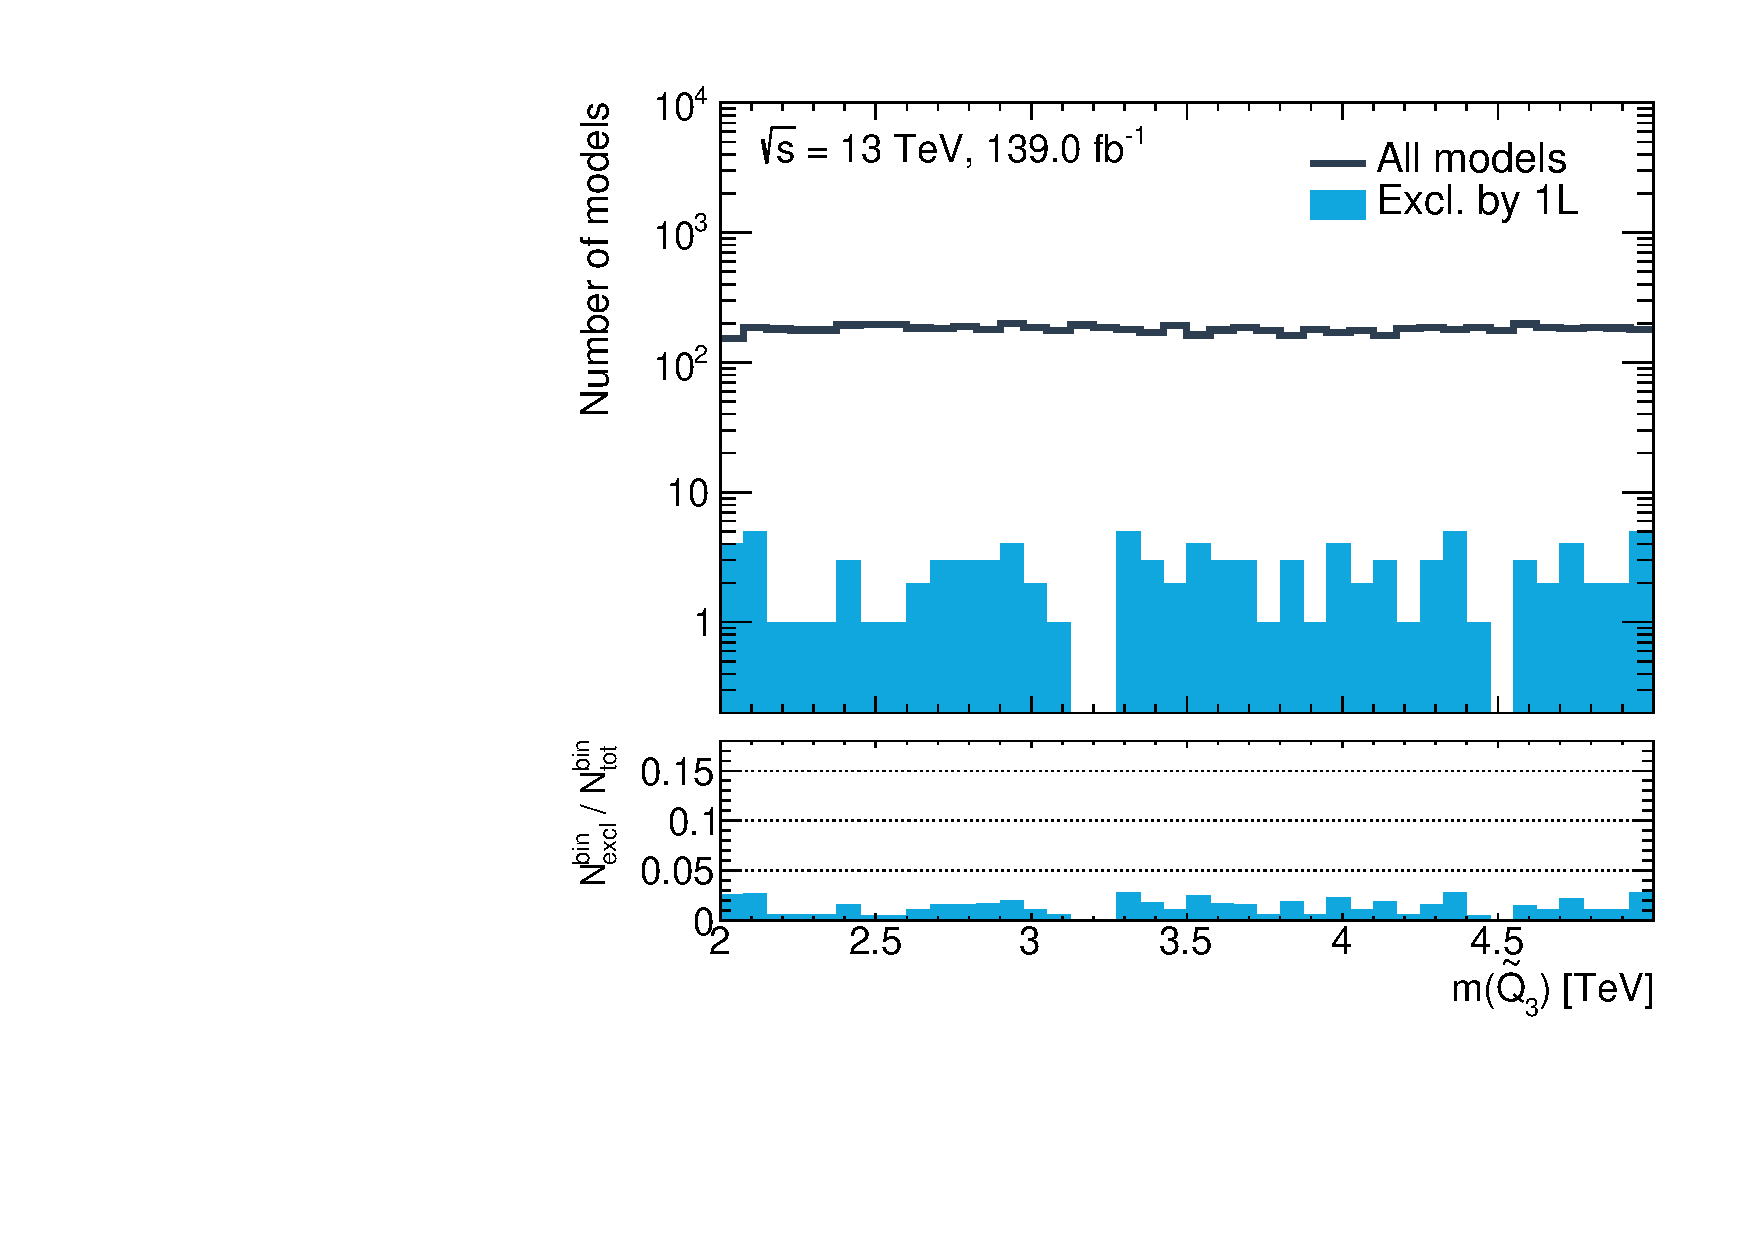
\includegraphics[width=\textwidth]{1D/mqL3}
	\end{subfigure}
	\caption{Bin-by-bin number of excluded models as a one-dimensional function of the remaining \gls{pmssm} parameters not already shown in \cref{fig:impact_pMSSM_parameters_1D}. The bin-wise fraction of excluded models, $N^\mathrm{bin}_\mathrm{excl} / N^\mathrm{bin}_\mathrm{total}$, is shown in the lower pad. All models are evaluated using the simplified likelihood of the \onelepton search.}
	\label{fig:impact_pMSSM_parameters_1D_2}
\end{figure}


\FloatBarrier

\section{Impact on dark matter relic density}

\Cref{fig:relic_density_lsp_withConstraint} compares the density of \gls{pmssm} models in a two-dimensional projection on the $\Omega_{\tilde{\chi}} h^2$--$m(\lsp)$ plane before and after the \gls{lep} constraint on the chargino mass of $m(\charg) > \SI{103.5}{\GeV}$~\cite{lep_susy_results} is applied. Only models with a bino-like \gls{lsp} provide a light \gls{lsp} with mass below $\SI{e2}{\GeV}$ after the \gls{lep} constraint. In order for the \textit{Z}- and \textit{h}-funnels to become visible, \ie for there to be a sizeable number of models with a light bino-like \gls{lsp} and $\Omega_{\tilde{\chi}} h^2 < 0.12$ c, the region with  $m(\lsp) > \SI{e2}{\GeV}$ would need to be oversampled. Due to the lack thereof within the scope of this thesis, only a small number of models with a bino-like \gls{lsp} and $\Omega_{\tilde{\chi}} h^2 < 0.12$ are sampled and subsequently evaluated using the \onelepton search.

\begin{figure}[h]
	\centering
	\begin{subfigure}[b]{0.49\linewidth}
		\centering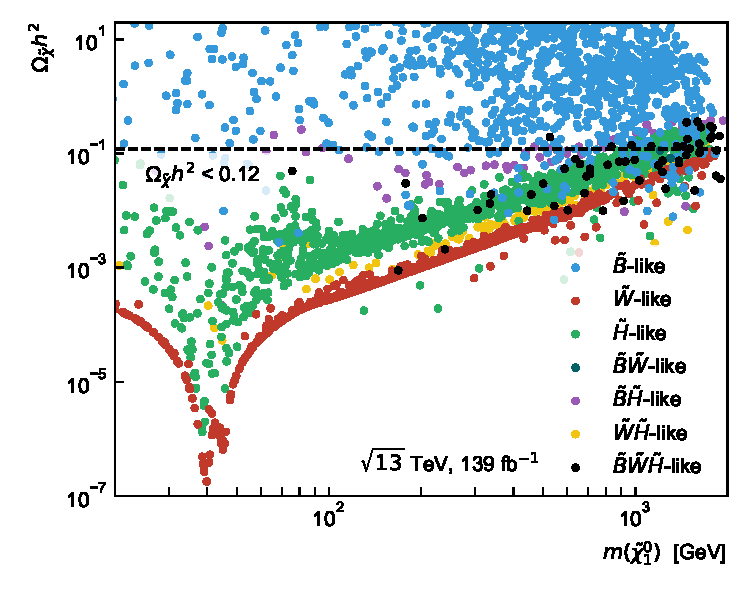
\includegraphics[width=\textwidth]{scatter/relic_density_lsp}
		\caption{Without LEP constraint\label{fig:relic_density_lsp_no_constraint}}
	\end{subfigure}\hfill
	\begin{subfigure}[b]{0.49\linewidth}
		\centering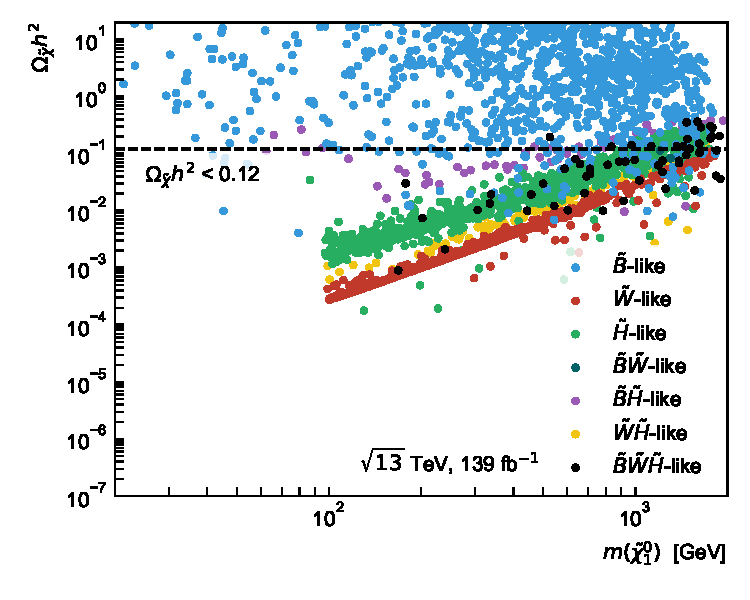
\includegraphics[width=\textwidth]{scatter/relic_density_lsp_limits}
		\caption{With LEP constraint\label{fig:relic_density_lsp_constraint}}
	\end{subfigure}\hfill
	\caption{Density of the \gls{pmssm} model points sampled in the plane spanned by the relic density and the $\lsp$ mass. The model points are additionally shown as a function of the nature of their $\lsp$. In fig.~\subref{fig:relic_density_lsp_no_constraint} all \gls{pmssm} models originally sampled and evaluated are shown. In fig.~\subref{fig:relic_density_lsp_constraint}, only models satisfying the constraint $m(\charg) > \SI{103.5}{\GeV}$ set by \gls{lep}~\cite{lep_susy_results} are shown. The horizontal dashed line represents the \gls{dm} relic density measurement by the Planck collaboration, interpreted as an upper limit $\Omega_{\tilde{\chi}} h^2 < 0.12$ such that the $\lsp$ can be a sub-dominant \gls{dm} component.}
	\label{fig:relic_density_lsp_withConstraint}
\end{figure}
